\documentclass[a4paper, 12pt]{article}

%%%%%%%%%%%%%%%%%%% Packages

%%%%% Tools

\usepackage{comment}
\usepackage{lipsum}
\usepackage{xstring}

%%%%% Document

\usepackage[pdfusetitle]{hyperref}

\usepackage{geometry}
\geometry{paper=a4paper,top=3.5cm,bottom=2.5cm,right=2.5cm,left=2.5cm}

\usepackage{fancyhdr}
\pagestyle{fancy}
\fancyhead[L]{}
\fancyhead[R]{\leftmark}
\fancyfoot[C]{\thepage}
\renewcommand{\headrulewidth}{0pt}

%%%%% Text

\usepackage[utf8]{inputenc}
\usepackage[T1]{fontenc}
\usepackage[parfill]{parskip}
\usepackage{csquotes}

\newlength{\mytextsize}
\makeatletter
\setlength{\mytextsize}{\f@size pt}
\makeatother

%%%%% Languages

\ifx\languages\undefined
	\usepackage[english, french]{babel}
\else
	\usepackage[\languages]{babel}
\fi

% english

\addto\captionsenglish{\def\figurename{Figure}}
\addto\captionsenglish{\def\tablename{Table}}

\newcommand{\st}{\text{s.t.}}

% french

\frenchbsetup{StandardLists=true}

\addto\captionsfrench{\def\figurename{Figure}}
\addto\captionsfrench{\def\tablename{Table}}
\addto\captionsfrench{\def\proofname{Preuve}}

\def\tq{\text{t.q.}}
\def\cad{c.-à-d. }
\def\Cad{C.-à-d. }

%%%%% Styles

\usepackage[skip=\mytextsize]{caption}
\usepackage{float}
\usepackage{mdframed}
\usepackage{enumitem}
\usepackage{eurosym}
\usepackage{color}

\newcommand\caaption[1]{\caption{#1}\vspace{-1\mytextsize}}

%%%%% Mathematics

\usepackage{amsmath}
\usepackage{amssymb}
\usepackage{amsfonts}
\usepackage{bm}
\usepackage{esint}
\usepackage[makeroom]{cancel}

\newcommand{\fact}[1]{#1!}
\newcommand{\e}[1]{\mathbf{e}_{#1}}
\newcommand{\deriv}{\mathrm{d}}
\DeclareMathOperator{\tr}{tr}


%%%%% SI units

\usepackage[squaren,Gray,cdot]{SIunits}
\usepackage{sistyle}

\IfStrEq{\languagename}{french}{
	\SIdecimalsign{,}
}

%%%%% Chemistry

\usepackage[version=4]{mhchem}

%%%%% Table & Figure

\usepackage{array}
\usepackage{tabularx}
\usepackage{multirow}
\usepackage{multicol}
\newcolumntype{M}[1]{>{\centering\arraybackslash}m{#1}}
%\setlength\extrarowheight{0em}
\renewcommand{\arraystretch}{1.3}

\usepackage{pgfplots}
\usepackage{tikz}
\usetikzlibrary{shapes.geometric, positioning}
\usepackage{graphics}
\usepackage{graphicx}
\pgfplotsset{axis on top, compat = 1.3}

%%%%%% Theorems and Definitions

\usepackage{amsthm}
\usepackage{thmtools}

\IfStrEq{\languagename}{english}{
	\def\lgthm{Theorem}
	\def\lglem{Lemma}
	\def\lgprop{Proposition}
	\def\lgdefn{Definition}
	\def\lghyp{Hypothesis}
	\def\lgquest{Question}
	\def\lgansw{Answer}
	\def\lgexpl{Example}
	\def\lgrmk{Remark}
	\def\lgnote{Note}
	\def\lgtip{Tip}
}

\IfStrEq{\languagename}{french}{
	\def\lgthm{Théorème}
	\def\lglem{Lemme}
	\def\lgprop{Proposition}
	\def\lgdefn{Définition}
	\def\lghyp{Hypothèse}
	\def\lgquest{Question}
	\def\lgansw{Réponse}
	\def\lgexpl{Exemple}
	\def\lgrmk{Remarque}
	\def\lgnote{Note}
	\def\lgtip{Conseil}
}

\theoremstyle{plain}
\newtheorem{thm}{\lgthm}[section]
\newtheorem{lem}{\lglem}[section]
\newtheorem{prop}{\lgprop}[section]

\theoremstyle{definition}
\newtheorem{defn}{\lgdefn}[section]
\newtheorem{hyp}{\lghyp}[section]
\newtheorem{quest}{\lgquest}[]

\declaretheorem[
name=\lgansw,
qed={\lower-0.3ex\hbox{$\triangle$}},
within=quest
]{answ}

\declaretheorem[
name=\lgexpl,
qed={\lower-0.3ex\hbox{$\triangle$}},
within=section
]{expl}

\theoremstyle{remark}
\newtheorem*{rmk}{\lgrmk}
\newtheorem*{note}{\lgnote}
\newtheorem*{tip}{\lgtip}

\begingroup
\makeatletter
\@for\theoremstyle:=definition,remark,plain\do{%
	\expandafter\g@addto@macro\csname th@\theoremstyle\endcsname{%
		\addtolength\thm@preskip\parskip
	}%
}
\endgroup

%%%% Others

\renewcommand{\qedsymbol}{$\blacksquare$}

\newcommand{\mytableofcontents}{
	\newpage
	\pagenumbering{roman}
	\tableofcontents
	\newpage
	\pagenumbering{arabic}
}

%%%%%%%%%%%%%%%%%%%

%%%%%%%%%%%%%%%%%%% Titlepage

\def\logopath{include/resources/pdf/logo_uliege.pdf}
\def\toptitle{Université de Liège}
\title{Projet -- Étude statistique}
\def\subtitle{Éléments de statistiques}
\def\authorhead{Groupe 14}
\author{Jean-Baptiste \textsc{Crismer} (s161640)\\François \textsc{Rozet} (s161024)\\}
\newcommand{\context}{3\up{ème} année de Bachelier Ingénieur civil}
\date{Année académique 2018-2019}

%%%%%%%%%%%%%%%%%%% Others

\usepackage{colortbl}
\usepackage{listings}

\def\ptsd{\textperthousand}

\def\lstbasicfont{\fontfamily{pcr}\selectfont}

\lstdefinestyle{MatLab}{
	language=Matlab,
	%%%%%%
	showstringspaces=false,
	extendedchars=true,
	tabsize=4,
	columns=fixed,
	%%%%%%
	breaklines=true,
	breakatwhitespace=true,
	prebreak=\space,
	%%%%%%
	basicstyle=\fontfamily{pcr}\footnotesize,
	keywordstyle=\color{blue!60!black},
	commentstyle=\itshape\color{green!40!black},
	stringstyle=\color[rgb]{.627,.126,.941},
	%%%%%%
	morekeywords={clearvars, addpath, rng, mod, ones, numel, cell, cellfun, table, fieldnames, readtable, array2table, histogram, scatter, daspect, boxplot, cdfplot, icdf, cdf, kstest2, randi, corr, cf, gap, hasIn, isIn, ks2stat},
	%%%%%%
	numbersep=0.5\mytextsize,
	numbers=left,
	numberstyle={\lstbasicfont\footnotesize},
	%%%%%%
	frame=single,
	rulecolor=\color{black},
	framexleftmargin=2\mytextsize,
	xleftmargin=2\mytextsize,
	captionpos=b,
	aboveskip=1\mytextsize,
	belowskip=1\mytextsize
}

\renewcommand{\thesubsection}{\thesection.\alph{subsection}}
\renewcommand{\thesubsubsection}{\roman{subsubsection}.}

%%%%%%%%%%%%%%%%%%%

\begin{document}
	\newgeometry{margin = 2.5cm}
\makeatletter
\begin{titlepage}
	\begin{minipage}[t][0.425\textheight][t]{\textwidth}
		\begin{center}
		    \ifx\toptitle\undefined
    		    \vfill
    		    \ifx\logopath\undefined
    		    \else
    			    \includegraphics[height=0.2125\textheight]{\logopath}
    			\fi
    		\else
    		    \ifx\logopath\undefined
    		    \else
    			    \includegraphics[height=0.15\textheight]{\logopath}
    			\fi
    			\vfill
    			{\huge \textsc{\toptitle}}
			\fi
			\vfill
		\end{center}
	\end{minipage}
	\vfill
	\begin{minipage}{\textwidth}
		\hspace{0.5em}
		\begin{mdframed}[linewidth = 2pt, innertopmargin = 1em, innerbottommargin = 1em, leftline = false, rightline = false]
			\begin{center}
				{\huge \bfseries \@title}
			\end{center}
		\end{mdframed}
		\hspace{0.5em}
	\end{minipage}
	\vfill
	\begin{minipage}[b][0.425\textheight][t]{\textwidth}
			\ifx\subtitle\undefined
			\else
			    \vspace{-0.5em}
			    \begin{center}
				    {\LARGE \subtitle}
				\end{center}
			\fi
			\vfill
			\ifx\rightauthor\undefined
			    \begin{center}
			        \ifx\authorhead\undefined
			        \else
		                {\large\it \authorhead\\[0.5em]}
		            \fi
			        {\large \@author}
			    \end{center}
			\else
			    \begin{minipage}[t]{0.5\textwidth}
			        \begin{flushleft}
			            \ifx\authorhead\undefined
			            \else
			                {\large\it \authorhead\\[0.5em]}
			            \fi
				        {\large \@author}
				    \end{flushleft}
				\end{minipage}
				\begin{minipage}[t]{0.5\textwidth}
				    \begin{flushright}
				        \ifx\rightauthorhead\undefined
			            \else
			                {\large\it \rightauthorhead\\[0.5em]}
			            \fi
				        {\large \rightauthor\\}
				    \end{flushright}
				\end{minipage}
			\fi
			\vfill
			\begin{center}
			    \ifx\context\undefined
			    \else
			        {\large \context \\[0.5em]}
			    \fi
			    {\large \@date}
			\end{center}
	\end{minipage}
\end{titlepage}
\makeatother
\restoregeometry
	\section{Analyse descriptive} \label{sec:Q1}
    Avant d'utiliser la base de données contenant la population, il faut l'importer. Le script \texttt{loadData}\footnote{Tous les scripts et fonctions utilisés et demandés sont fournis en annexe.} a été écrit à cette fin et est dès lors appelé dans tous les autres. Si la matrice \texttt{f} (cf. section \ref{sec:Modularité}) est définie lors de son appel, les statistiques qu'elle contient seront alors calculées et stockées dans la structure \texttt{stats.dataset}.
	\subsection{Histogrammes} \label{sec:Q1a}
	Pour réaliser les histogrammes des taux de natalité et mortalité, on utilise la fonction \texttt{histogram} sur leur ensemble de données respectif. \par
	En observant l'histogramme\footnote{Les figures de ce document étant générées automatiquement à partir de la base de données, leurs axes sont en anglais.} du taux\footnote{Dans ce document les taux, ainsi que certains de leurs estimateurs, sont définis par mille habitants. Par la suite, si aucune unité n'est précisée pour un taux ou un estimateur, c'est qu'il est exprimé en \ptsd.} de natalité, on semble observer une décroissance exponentielle. Il se peut, néanmoins, que cette dernière corresponde à la partie décroissante d'une loi Gaussienne. À l'inverse, l'histogramme du taux de mortalité est assimilable à une gaussienne. \par
	\begin{figure}[h]
		\centering
		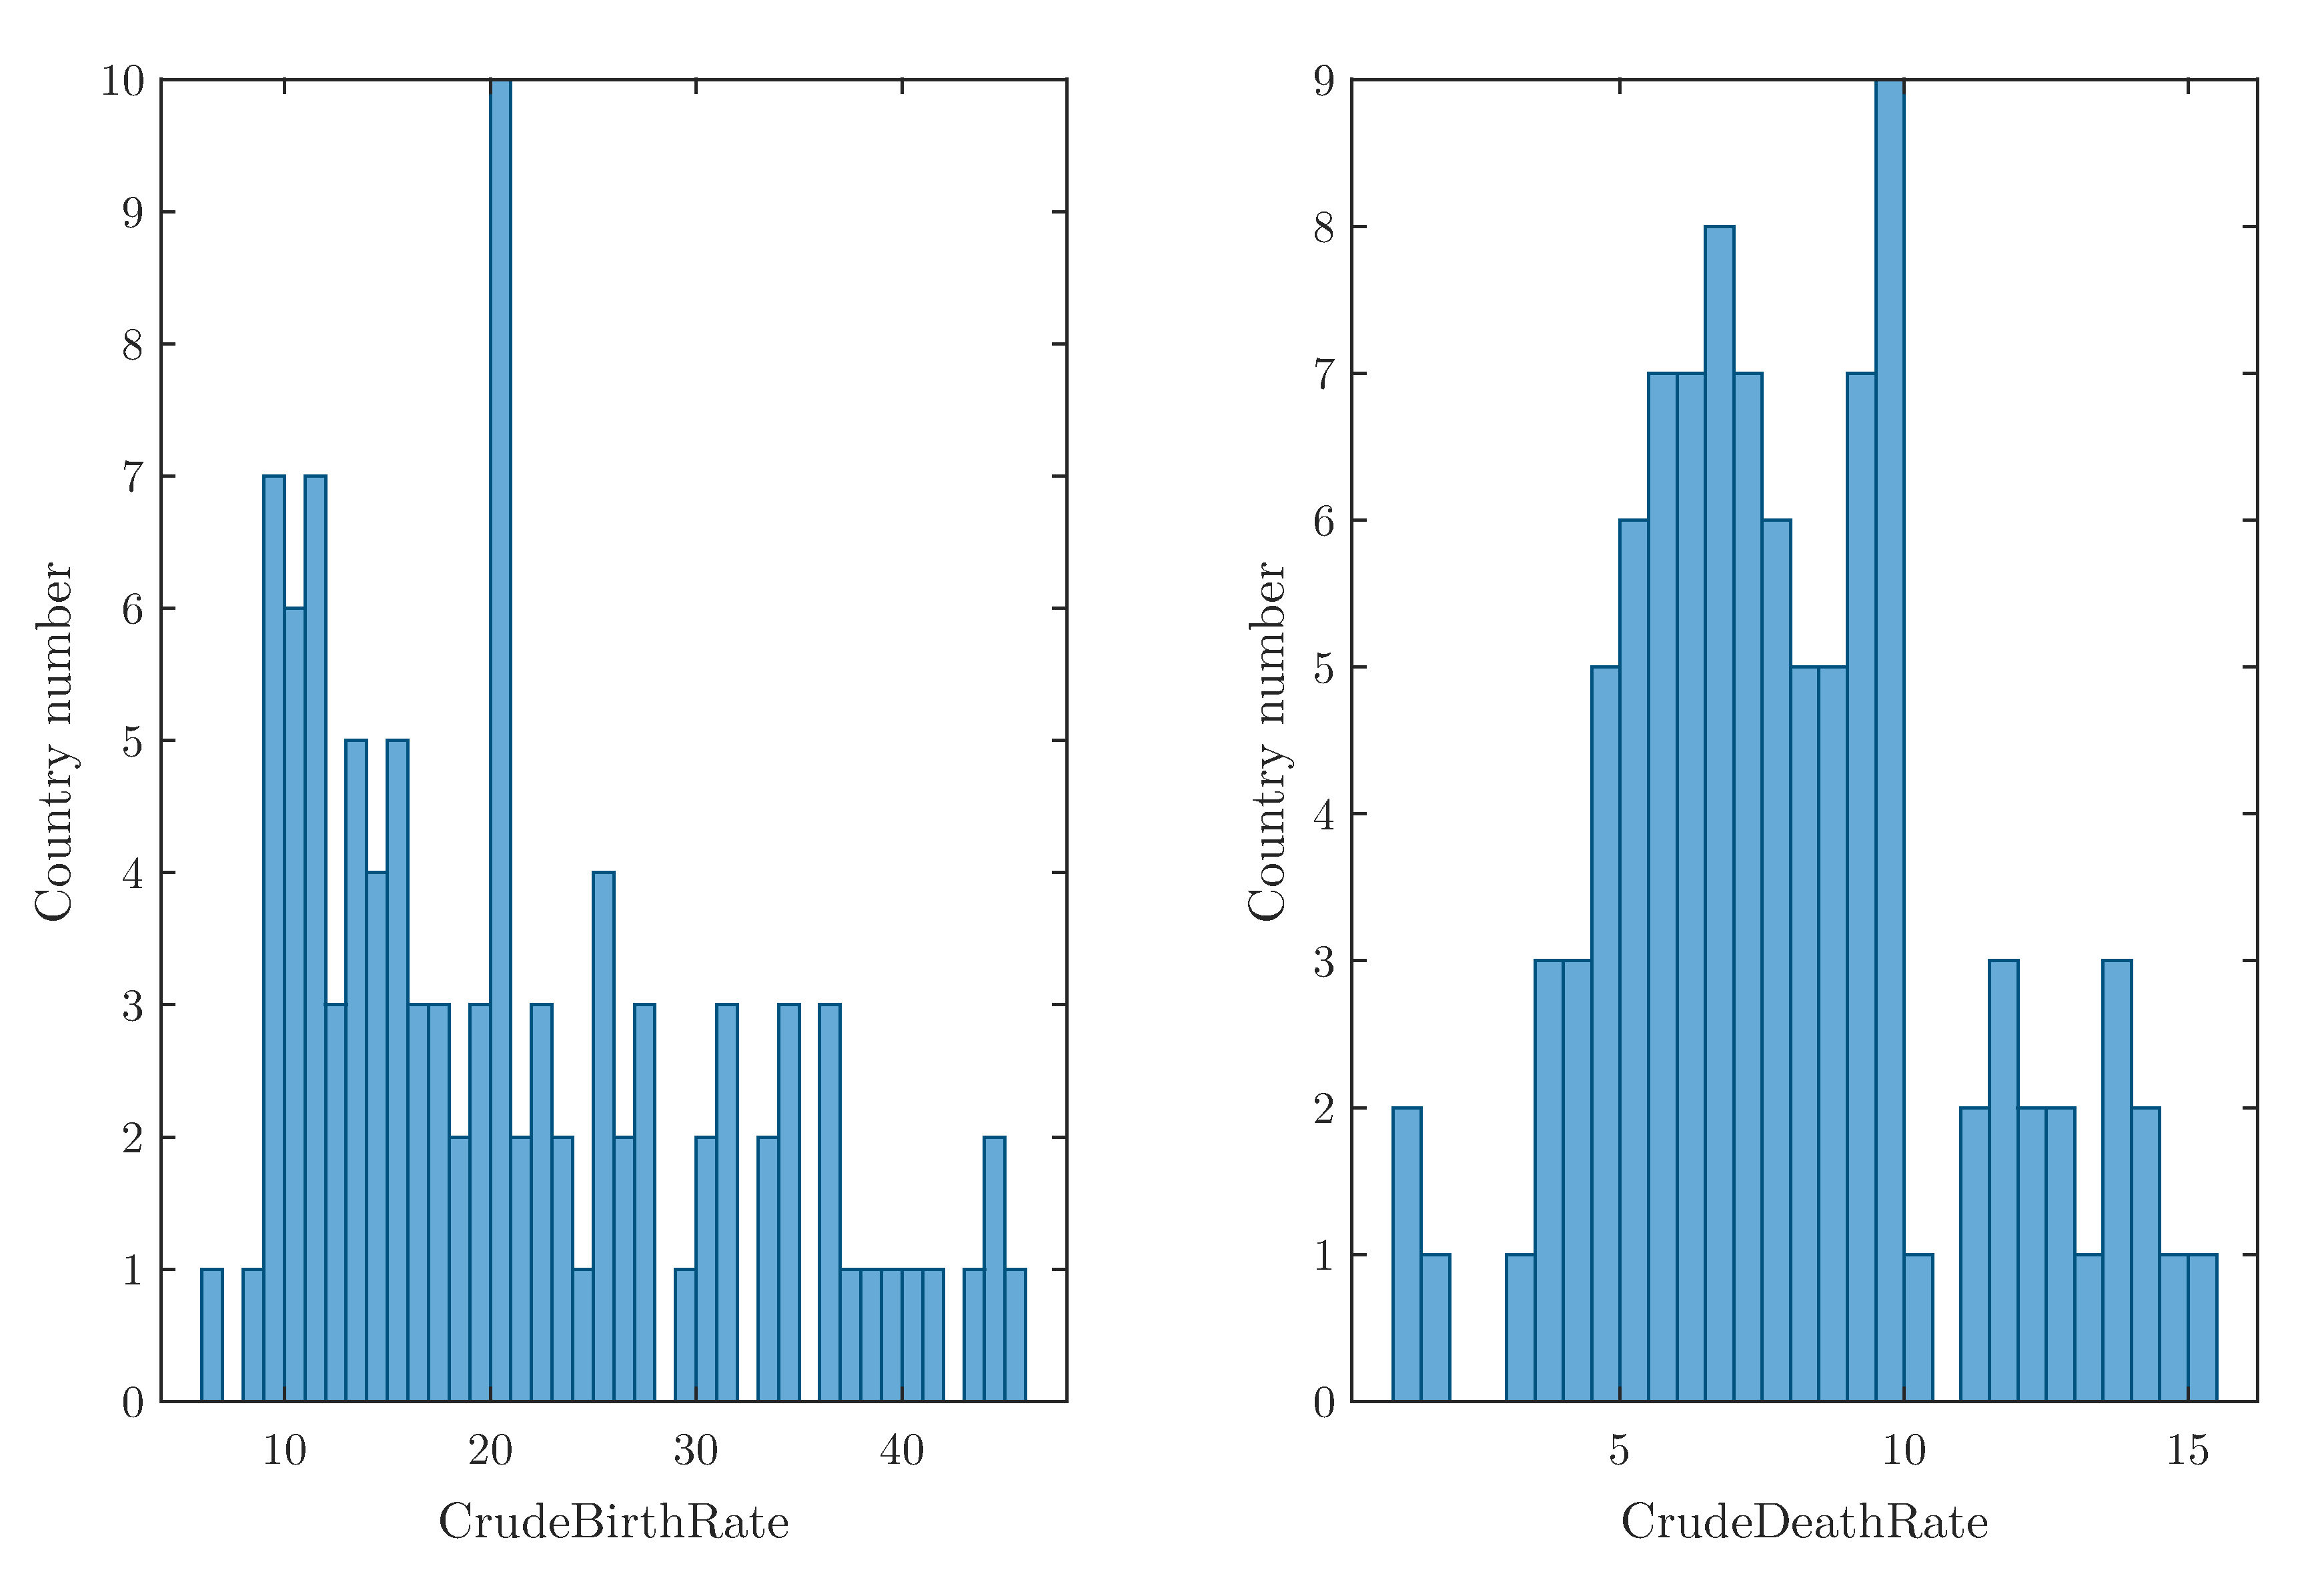
\includegraphics[scale=0.24]{resources/pdf/q1a.pdf}
		\caption{Histogrammes des taux de natalité et de mortalité.}
		\label{figure:Q1a}
	\end{figure}
	On peut noter que le taux de natalité, ou plutôt ses valeurs les plus fréquentes, est plus important que le taux de mortalité. Cela se traduit, d'un point de vue démographique, par un accroissement général de population. On remarque aussi que la fréquence associée aux valeurs du taux de natalité comprise entre $20$ et $21$ s'écarte fortement de la tendance générale.
	\subsection{Statistiques} \label{sec:Q1b}
	Pour calculer les statistiques moyenne, médiane, mode et écart-type on stocke respectivement les fonctions \texttt{mean}, \texttt{median}, \texttt{mode} et \texttt{std}, pré-implémentées dans \textsc{MATLAB}, dans la matrice \texttt{f} (cf. section \ref{sec:Q1}). \par
	Se trouvant dans la table \ref{table:Q1b}, ces statistiques calculées pour les taux de natalité et mortalité de toute la population, permettent d'observer que la moyenne et la médiane sont relativement peu distante. Dès lors, les valeurs aberrantes sont soit réparties équitablement autour de la moyenne soit absentes. La seconde hypothèse sera validée plus tard. \par
	À l'inverse, même s'il vaut la valeur la plus représentée, le mode estime très mal les valeurs les plus communes. On remarque aussi que l'écart-type, et dès lors la variance, est relativement important ce qui traduit un grand étalement des données autour de la moyenne. \par
	\begin{table}[h]
		\centering
		\begin{tabular}{|c|c|c|c|c|}
			\hline
			  Taux    & Moyenne [\ptsd] & Médiane [\ptsd] &  Mode [\ptsd]  & Écart-type [\ptsd] \\ \hline\hline
			Natalité  & $\num{21.284}$  & $\num{19.900}$  & $\num{10.700}$ &   $\num{9.952}$    \\ \hline
			Mortalité &  $\num{7.866}$  &  $\num{7.450}$  & $\num{5.700}$  &   $\num{3.008}$    \\ \hline
		\end{tabular}
		\caption{Statistiques sur les taux de natalité et mortalité de la population.}
		\label{table:Q1b}
	\end{table}
	Ce tableau permet aussi de mettre en évidence que les taux de natalité ($\num{11.7}$) et de mortalité ($\num{9.9}$) de la Belgique sont respectivement inférieur et supérieur à leur moyenne respective. On en déduit que la Belgique possède un accroissement démographique parmi les plus bas de la population.
	\subsection{Taux normaux} \label{sec:Q1c}
	Un individu d'une population est défini comme normal au sens de la loi normale s'il appartient à l'intervalle $\left[\mu - \sigma;\, \mu + \sigma\right]$, où $\mu$ et $\sigma$ sont respectivement la moyenne et l'écart-type de la population. Dès lors, un taux de natalité, respectivement mortalité, est normal s'il appartient à $\left[\num{11.282};\, \num{31.286}\right]$, respectivement $\left[\num{4.843};\, \num{10.889}\right]$. \par
	Ainsi, la Belgique est considérée comme normale au sens de la loi normale tant en natalité, qu'en mortalité. \par
	Pour statuer de la normalité des autres pays, on écrit la fonction \texttt{isIn} qui détermine si une valeur est contenue dans un intervalle ou non. On compte ainsi que $63 \%$ des pays ont un taux de natalité normal et que $68 \%$ ont un taux de mortalité normal.
	\subsection{Boîtes à moustaches} \label{sec:Q1d}
	Pour réaliser les boîtes à moustaches des taux de natalité et mortalité, on utilise la fonction \texttt{boxplot} sur leur ensemble de données respectif. \par
	\begin{figure}[h]
		\centering
		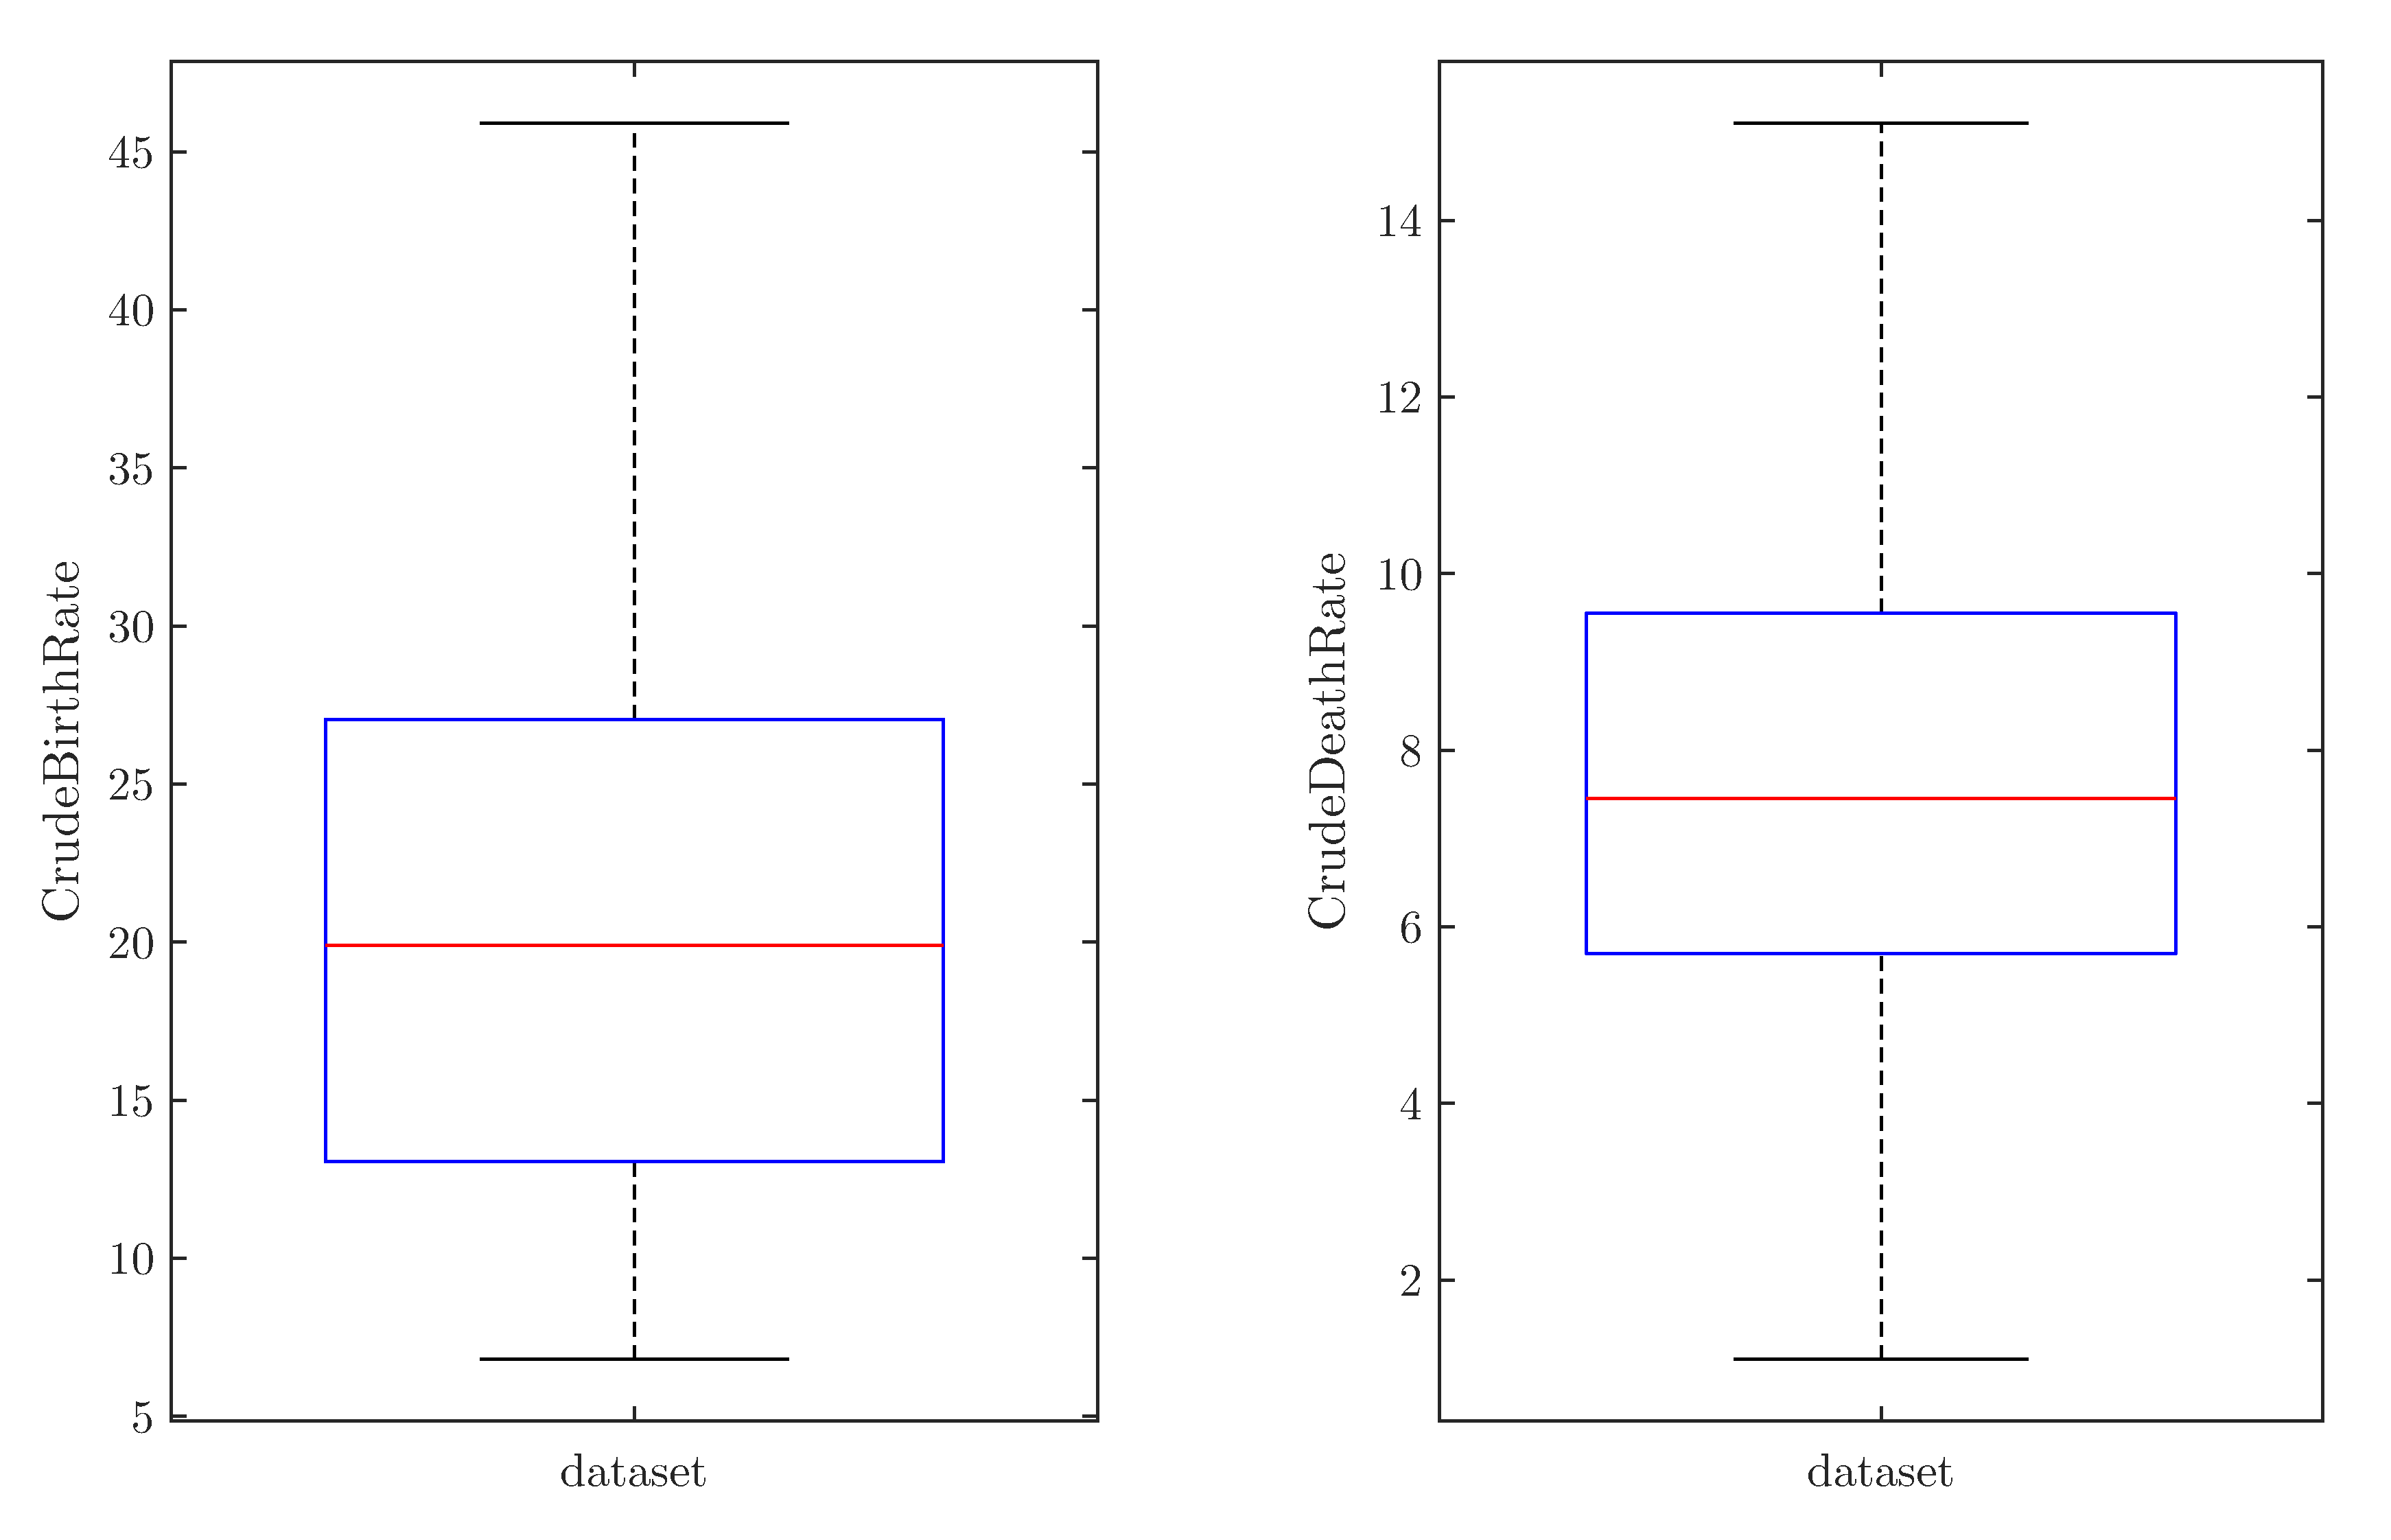
\includegraphics[scale=0.24]{resources/pdf/q1d.pdf}
		\caption{Boîtes à moustaches des taux de natalité et mortalité.}
		\label{figure:Q1d}
	\end{figure}
	La figure \ref{figure:Q1d} permet de noter l'absence de données aberrantes. S'il y en avait, elles seraient marquées de croix rouges. \par
	Les quartiles retranscrits dans la table \ref{table:Q1d}, sont, quant à eux, calculés à partir de la fonction \texttt{quantile}. \par
	\begin{table}[h]
		\centering
		\begin{tabular}{|c|c|c|c|}
			\hline
			\multirow{2}{*}{Taux} &    \multicolumn{3}{c|}{Quartile [\ptsd]}     \\ \cline{2-4}
			                      &   1\up{er}    &  2\up{ème}   &   3\up{ème}   \\ \hline\hline
			      Natalité        & $\num{13.05}$ & $\num{19.9}$ & $\num{27.05}$ \\ \hline
			      Mortalité       &  $\num{5.7}$  & $\num{7.45}$ & $\num{9.55}$  \\ \hline
		\end{tabular}
		\caption{Quartiles des taux de natalité et mortalité.}
		\label{table:Q1d}
	\end{table}
	Ils correspondent effectivement aux valeurs observables dans les boîtes à moustaches. On note aussi que la Belgique se trouve dans les $25\%$ les plus bas en natalité et les plus haut en mortalité.
	\subsection{Polygones des fréquences cumulées} \label{sec:Q1e}
	Repris dans la figure \ref{figure:Q1e}, les polygones des fréquences cumulées, tracés à l'aide de la fonction \texttt{cdfplot}, permettent de statuer à propos de la distribution des taux. Si une loi normale est faiblement discernable pour le taux de mortalité, ce n'est pas le cas pour le taux de natalité. \par
	\begin{figure}[h]
		\centering
		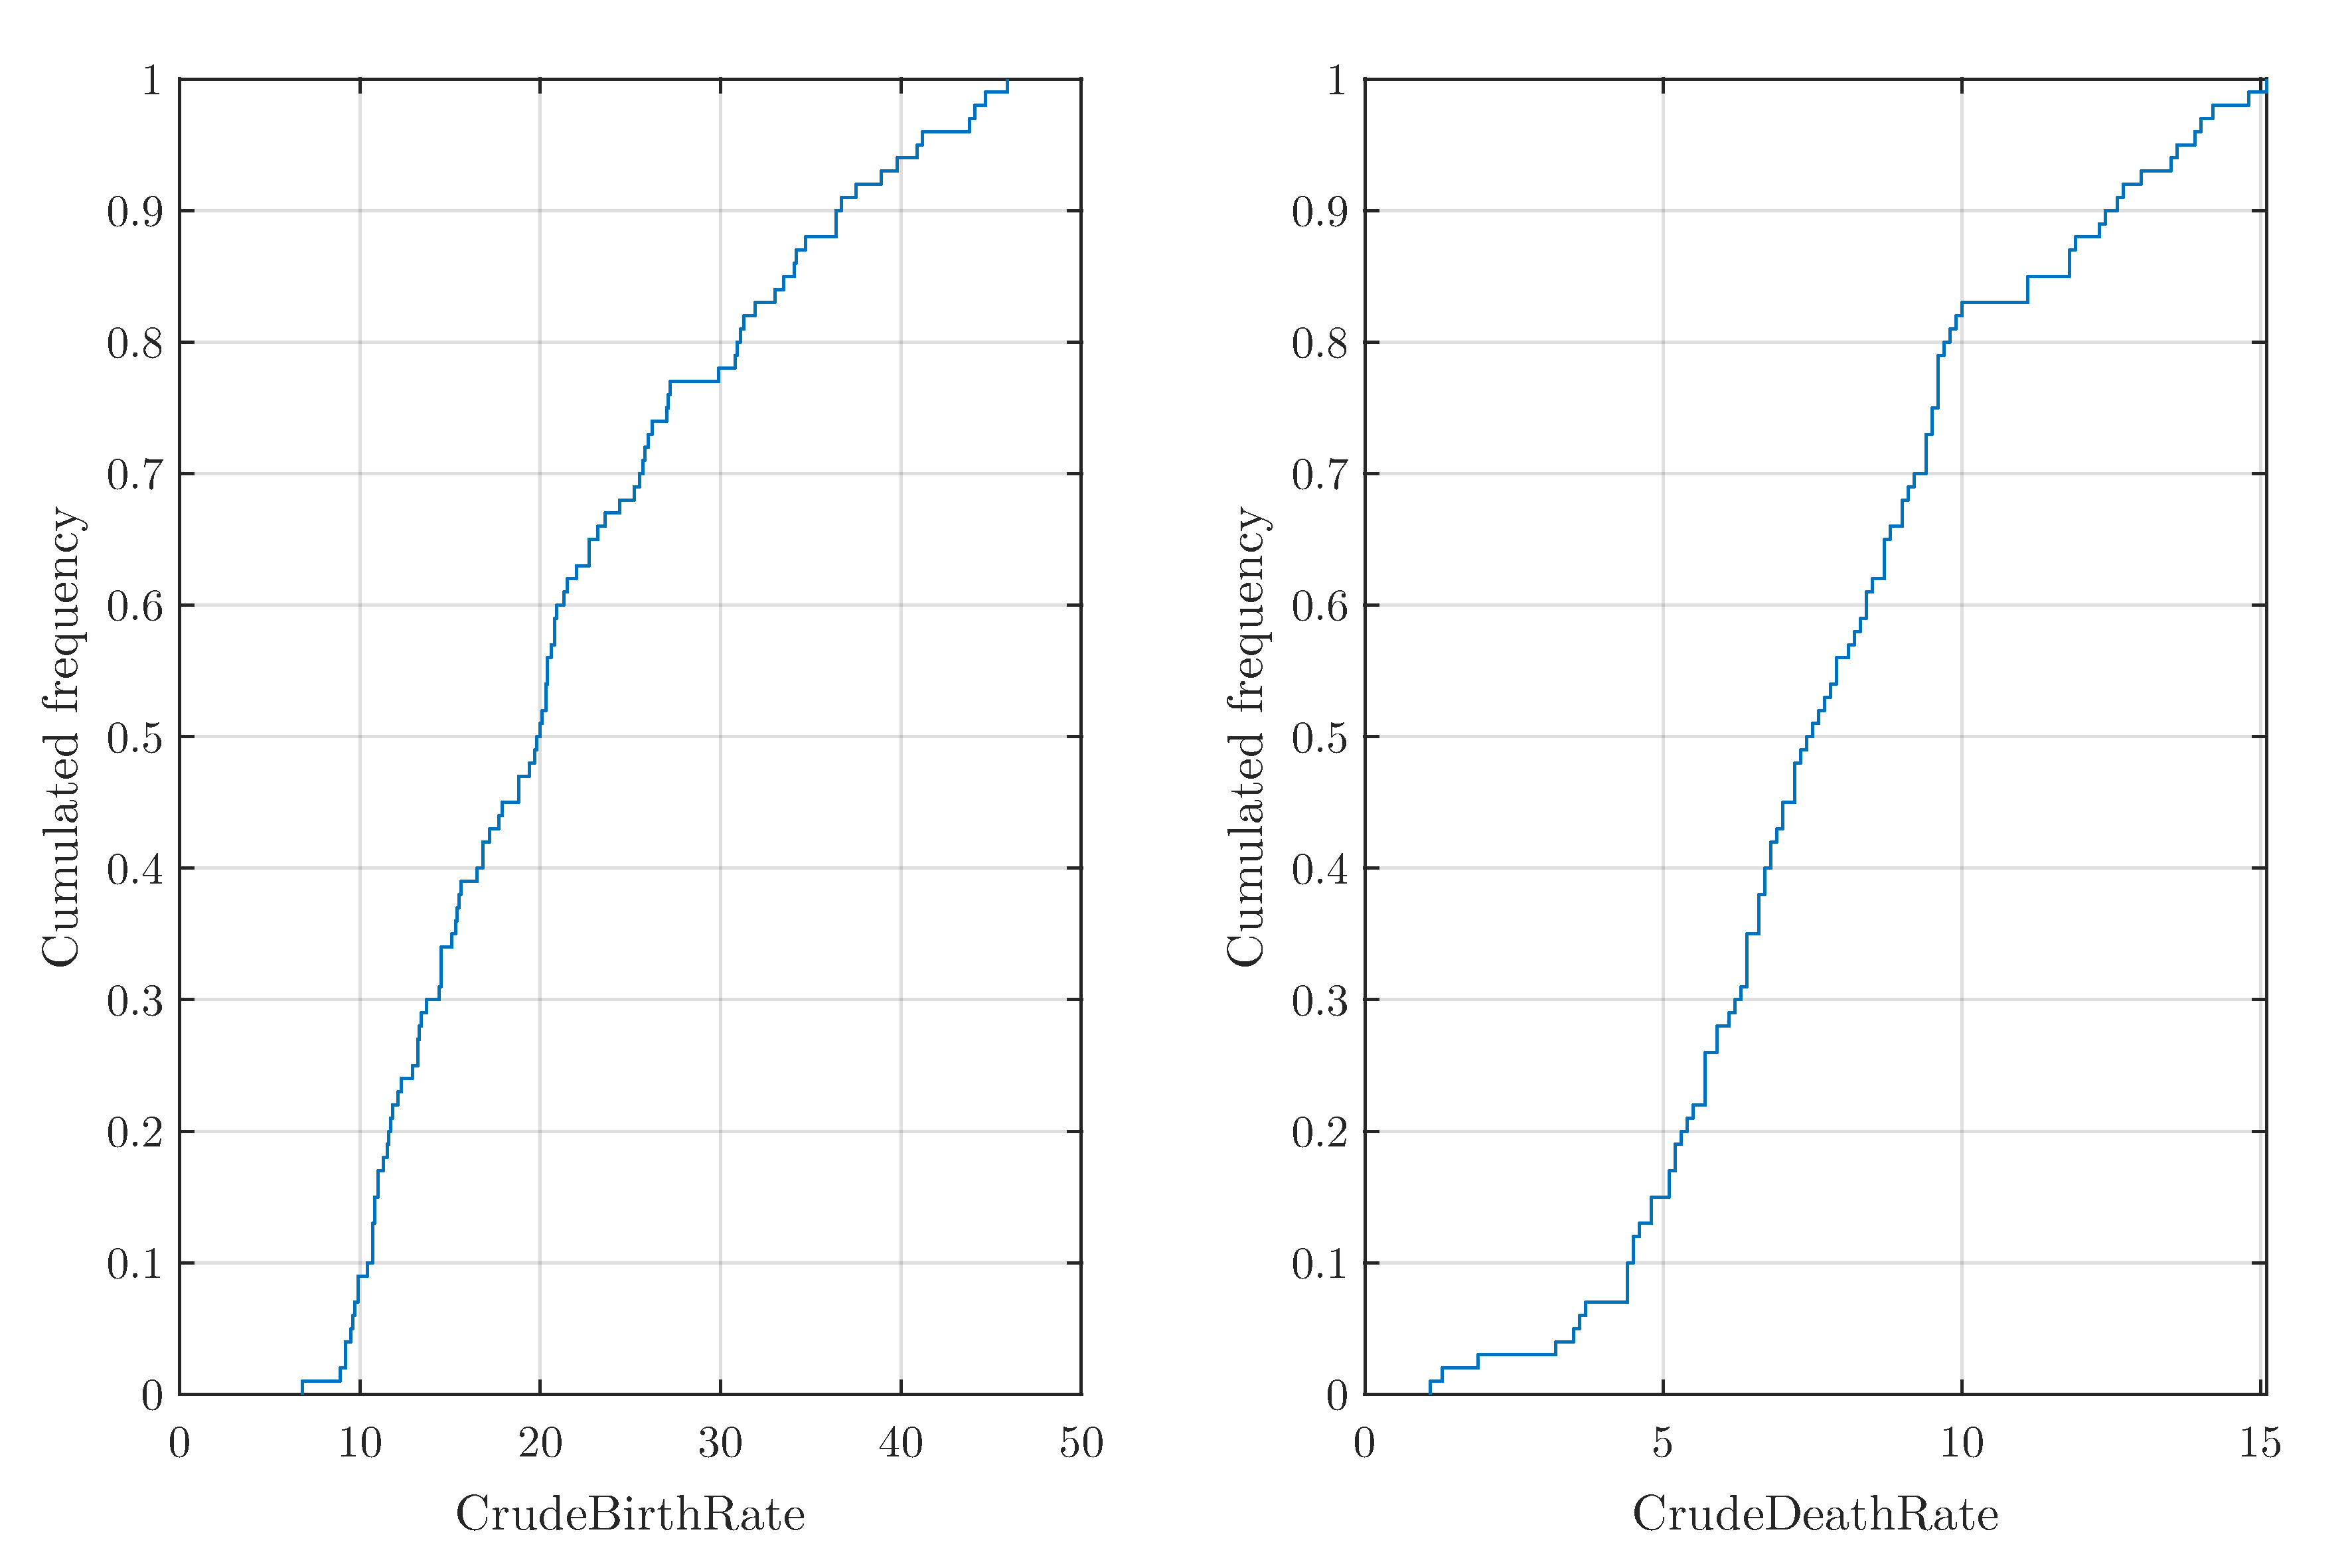
\includegraphics[scale=0.24]{resources/pdf/q1e.pdf}
		\caption{Polygones des fréquences cumulées des taux de natalité et de mortalité.}
		\label{figure:Q1e}
	\end{figure}
    Pour calculer la proportion de pays ayant un taux de natalité inférieur ou égal à $20$ et supérieur à celui de la Belgique, noté $b$, on écrit et utilise la fonction \texttt{cf} qui détermine la fréquence cumulée (\cad la proportion de valeurs inférieures ou égales) associée à une valeur $x$ dans une population $D_{n}$. Ainsi, il suffit de soustraire la fréquence cumulée de la Belgique à celle de $20$ pour trouver la proportion recherchée.
    \begin{align*}
        P(b < x \leq 20) & = P(x \leq 20) - P(x \leq b) \\
                         & = \num{0.3}
    \end{align*}
	\subsection{Corrélation} \label{sec:Q1f}
	Le coefficient de corrélation entre les taux de natalité et mortalité, calculé à partir de la fonction \texttt{corr}, vaut $\num{0.1609}$. Ce résultat, assez faible, traduit une quasi-absence de corrélation entre les taux de natalité et mortalité. \par
	Cette interprétation est renforcée par la figure \ref{figure:Q1f}. En effet, il est difficile d'y observer une quelconque relation entre les deux taux. \par
	\begin{figure}[h!]
		\centering
		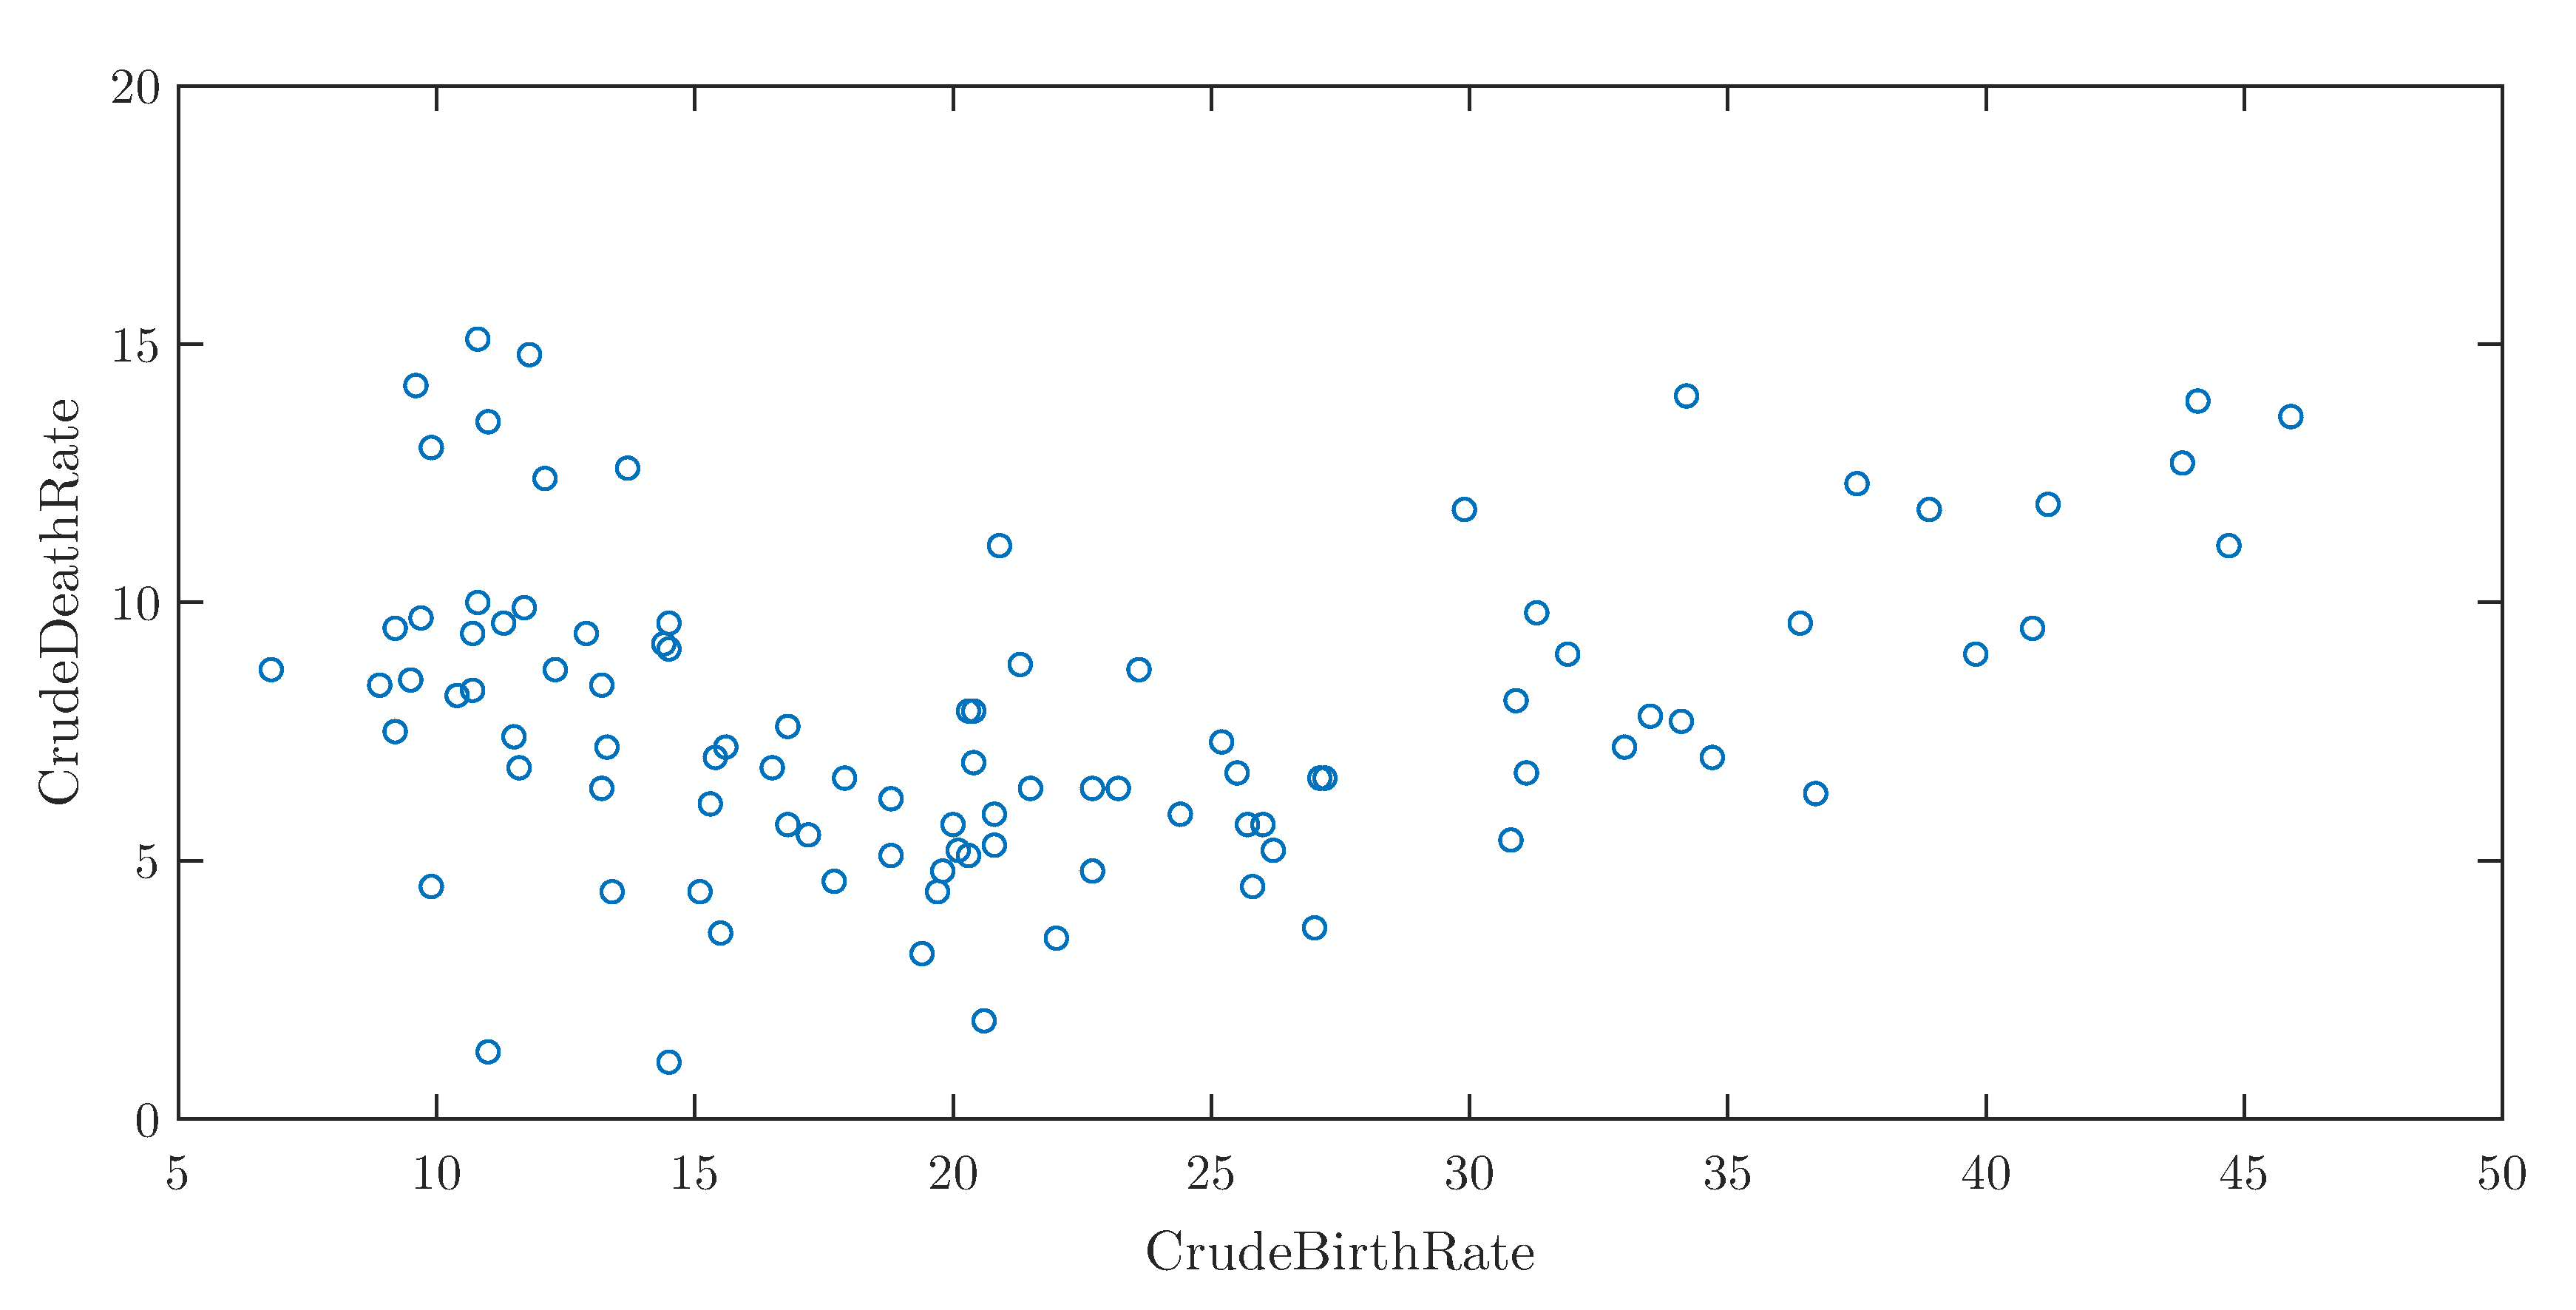
\includegraphics[scale=0.24]{resources/pdf/q1f.pdf}
		\caption{Nuage de points du taux de mortalité en fonction du celui de natalité.}
		\label{figure:Q1f}
	\end{figure}
    On peut néanmoins noter la légère tendance des pays ayant un taux de natalité élevé à également posséder un taux de mortalité élevé. Cela pourrait correspondre aux pays du tiers-monde.
	\section{Génération d'échantillons i.i.d.} \label{sec:Q2}
	Pour tirer les échantillons, le script \texttt{pickSamples} a été implémenté. De la même manière que \texttt{loadData} (cf. section \ref{sec:Q1}), il calculera, pour chaque échantillon i.i.d. tiré, les statistiques contenues dans la matrice \texttt{f} et les stockera dans \texttt{stats.sample}.
	\subsection{Un échantillon de vingt pays} \label{sec:Q2a}
	\subsubsection{Statistiques} \label{sec:Q2ai}
	Les statistiques de chaque échantillon sont obtenues par le script \texttt{Q2ai} de la même manière que celles de la population à la section \ref{sec:Q1b}. Comme le montre la table \ref{table:Q2ai}, les statistiques pour plusieurs échantillons restent relativement proches de celles calculées pour la population. Les écarts sont dûs aux pertes d'informations, résultat inévitable d'un échantillonnage. \par
	\begin{table}[h!]
		\centering
		\begin{tabular}{|c|c|c|c|c|}
			\hline
			Échantillon &            Taux            & Moyenne [\ptsd] & Médiane [\ptsd] & Écart-type [\ptsd] \\ \hline\hline
			    $1$     & \multirow{3}{*}{Natalité}  & $\num{20.795}$  &  $\num{20.7}$   &   $\num{7.1825}$   \\ \cline{1-1}\cline{3-5}
			    $2$     &                            & $\num{23.015}$  &  $\num{20.2}$   &   $\num{10.771}$   \\ \cline{1-1}\cline{3-5}
			    $3$     &                            &  $\num{20.94}$  &  $\num{19.7}$   &   $\num{10.222}$   \\ \hline\hline
			    $1$     & \multirow{3}{*}{Mortalité} &  $\num{7.68}$   &  $\num{8.45}$   &   $\num{2.7228}$   \\ \cline{1-1}\cline{3-5}
			    $2$     &                            &  $\num{7.715}$  &  $\num{7.30}$   &   $\num{3.8209}$   \\ \cline{1-1}\cline{3-5}
			    $3$     &                            &  $\num{7.905}$  &  $\num{8.00}$   &   $\num{2.9197}$   \\ \hline
		\end{tabular}
		\caption{Statistiques des taux de natalité et mortalité pour trois échantillons.}
		\label{table:Q2ai}
	\end{table}
	\subsubsection{Boîtes à moustaches} \label{sec:Q2aii}
	À l'instar de la section \ref{sec:Q1d}, les boîtes à moustaches sont dessinées par la fonction \texttt{boxplot} dans le script \texttt{Q2aii}. \par
	\begin{figure}[h!]
		\centering
		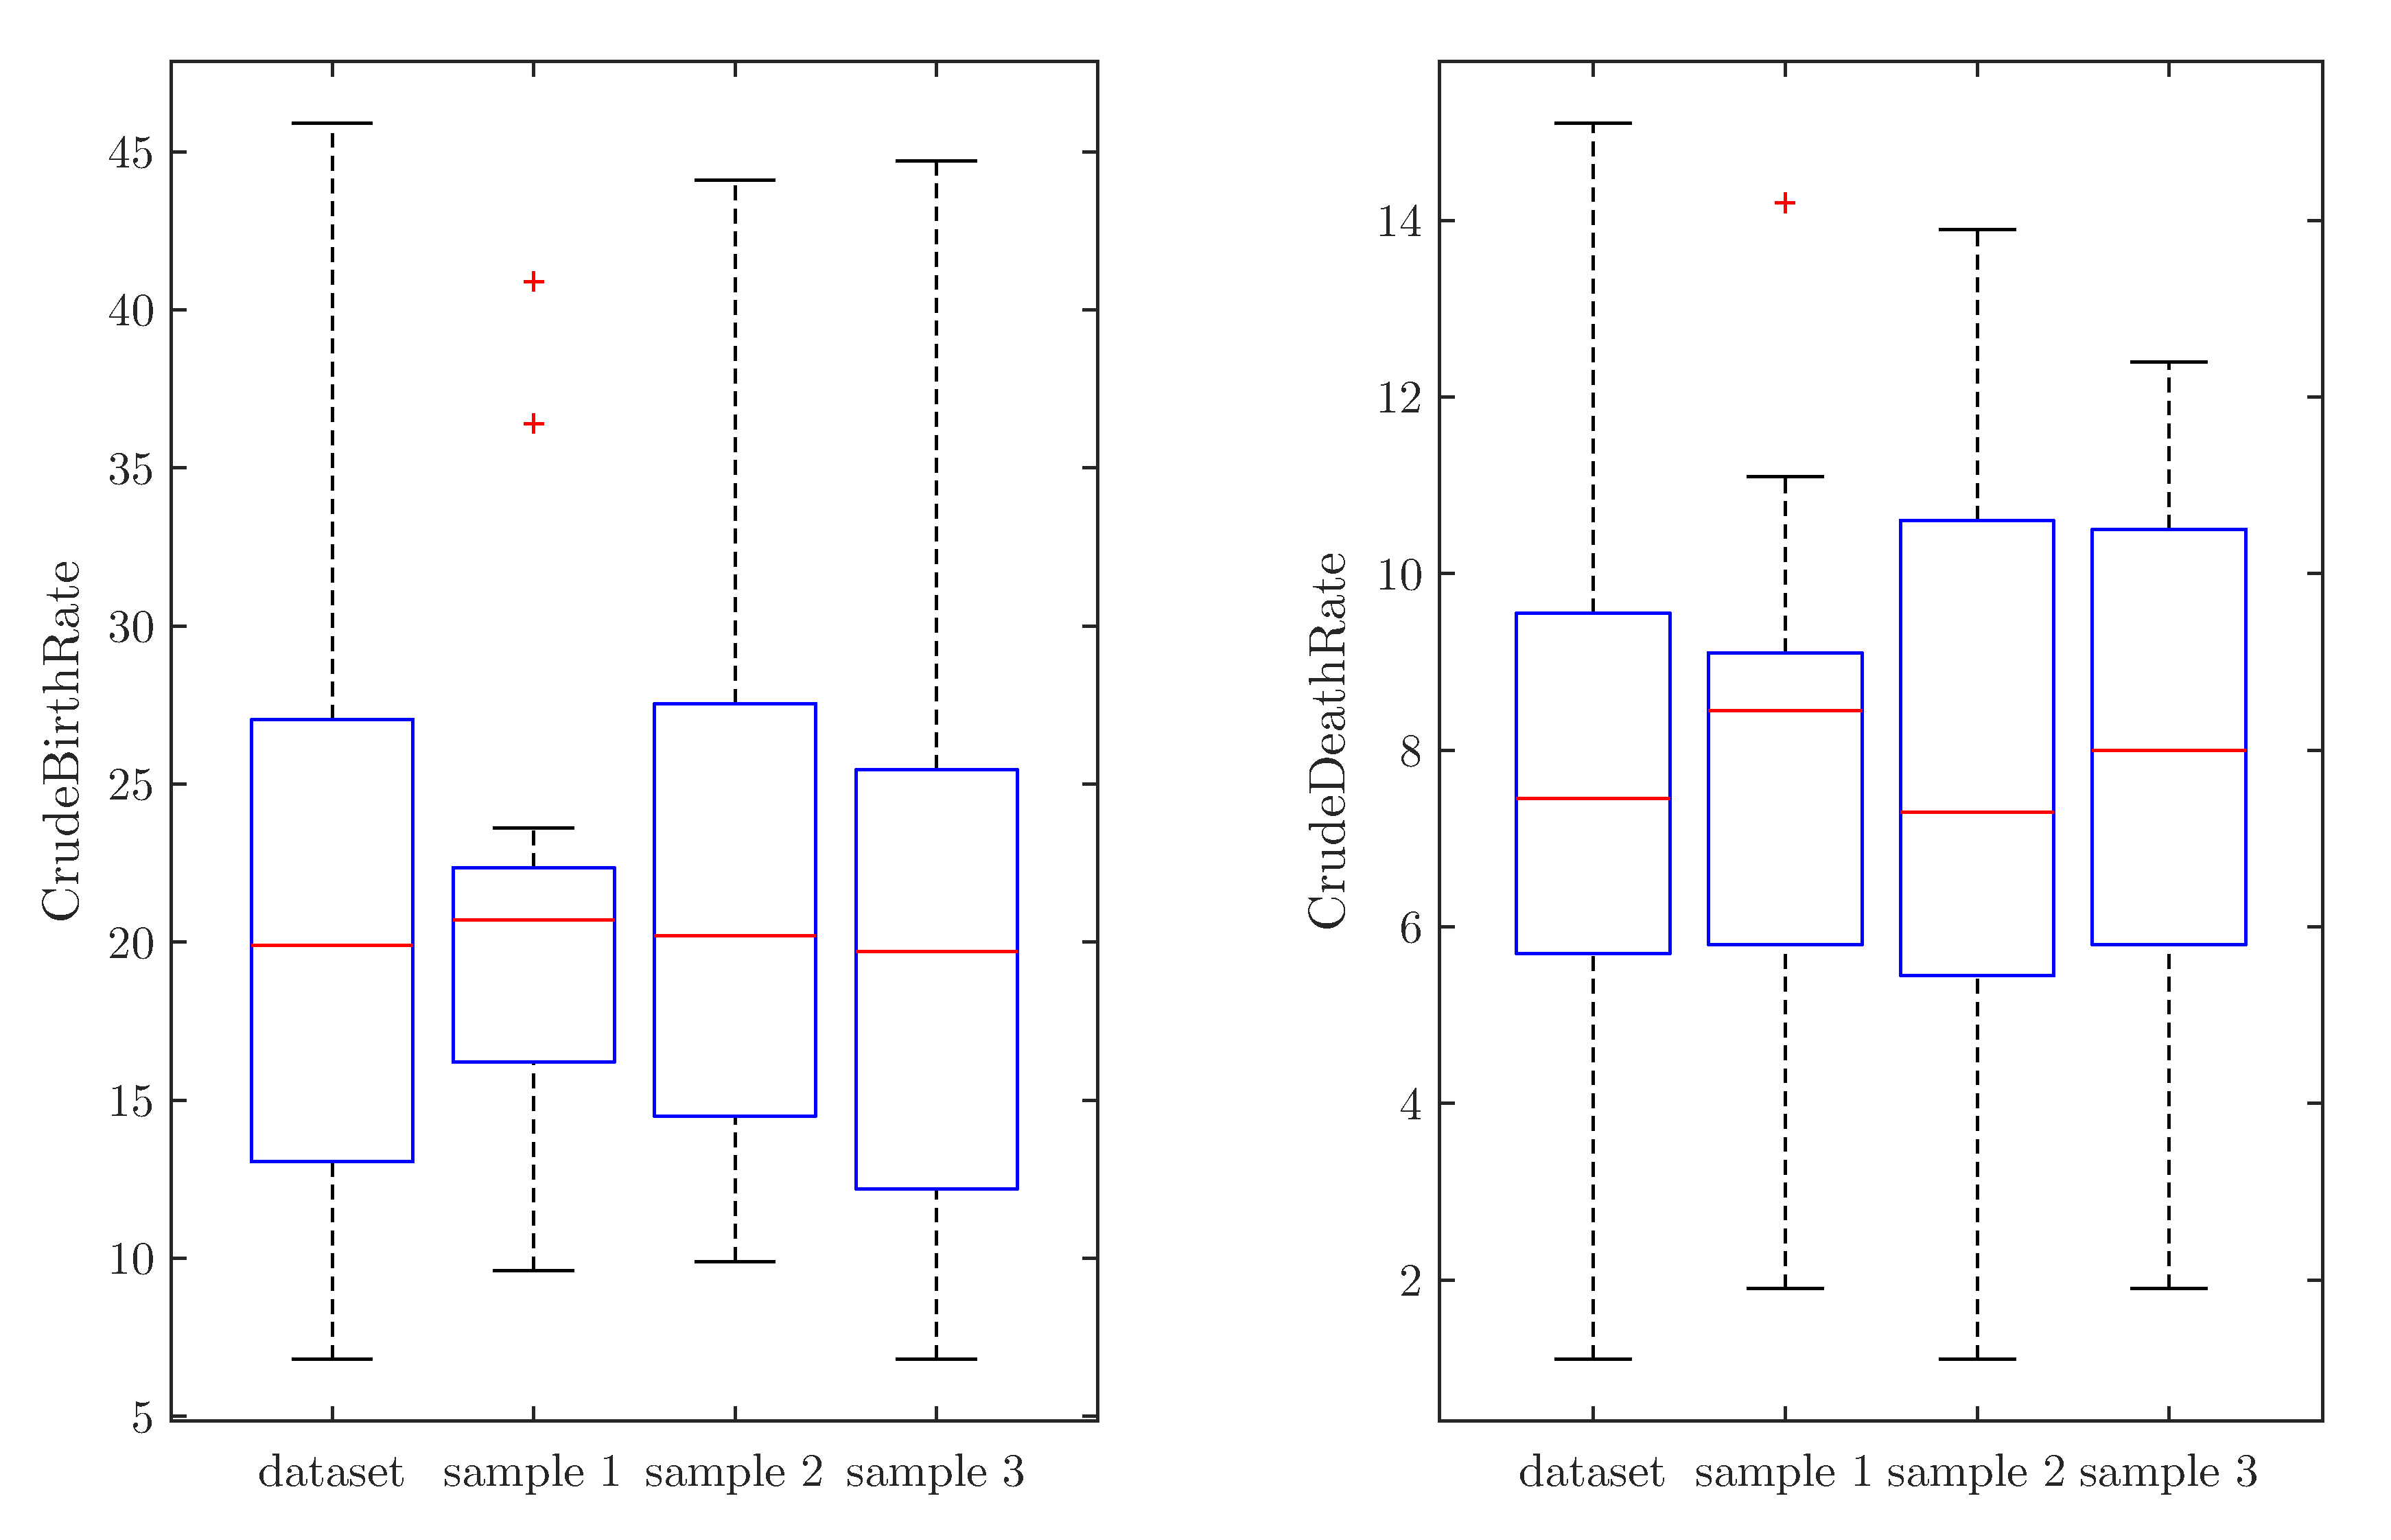
\includegraphics[scale=0.24]{resources/pdf/q2aii.pdf}
		\caption{Boîtes à moustaches des taux de natalité et mortalité pour la population et trois échantillons.}
		\label{figure:Q2aii}
	\end{figure}
	On note, à nouveau, quelques différences entre les échantillons et la population. La plus notable est que, contrairement à la population, les échantillons comportent des valeurs aberrantes. La deuxième, évidente, est que les moustaches des échantillons sont toujours comprises entre celles de la population. La dernière est, qu'en général, la médiane des échantillons reste relativement proche de la médiane de la population contrairement aux quartiles $25$ et $75$ qui fluctuent sensiblement.
	\subsubsection{Polygones de fréquences cumulées} \label{sec:Q2aiii}
	De la même manière qu'à la section \ref{sec:Q1e}, les polygones des fréquences cumulées, pour la population et les échantillons, sont tracés à l'aide de la fonction \texttt{cdfplot} par le script \texttt{Q2aiii}. \par
	\begin{figure}[h!]
		\centering
		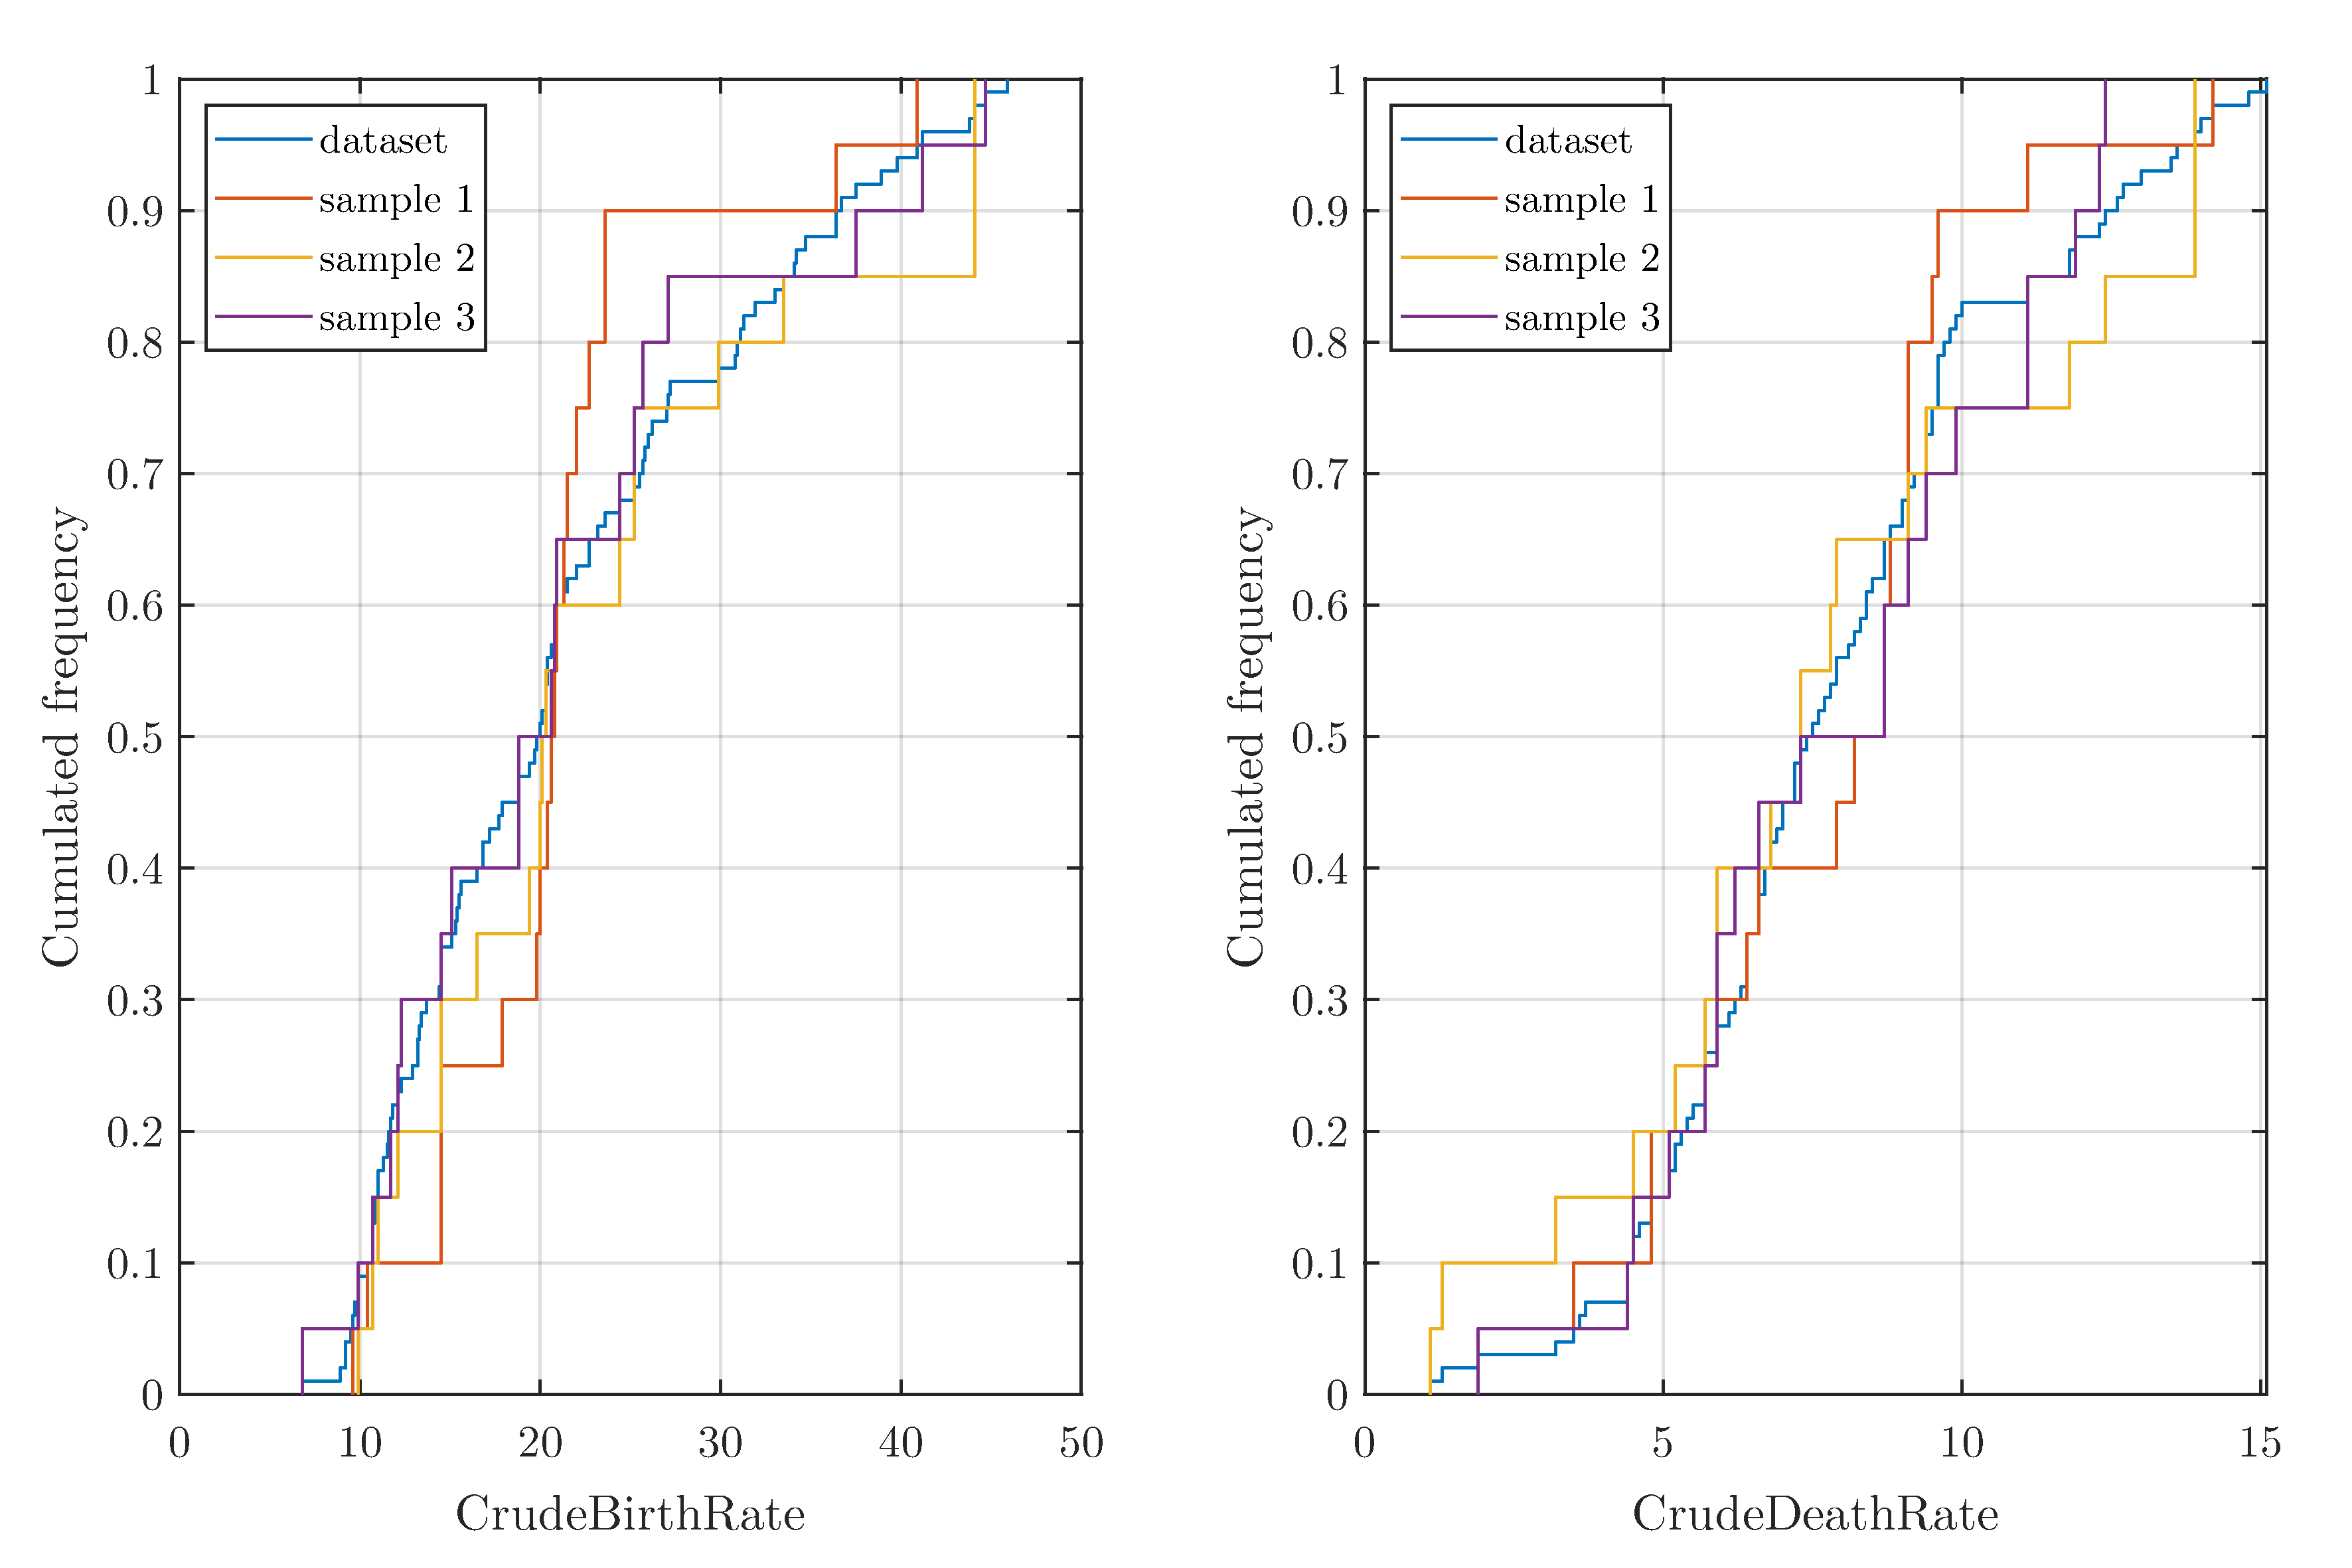
\includegraphics[scale=0.24]{resources/pdf/q2aiii.pdf}
		\caption{Polygone des fréquences cumulées des taux de natalité et mortalité pour la population et trois échantillons.}
		\label{figure:Q2aiii}
	\end{figure}
	On remarque dans la figure \ref{figure:Q2aiii} que la distribution des échantillons est moins régulière que celle de la population en ce sens qu'elle comporte de plus grandes \og{}marches\fg{}. Elle s'en éloigne aussi de façon significative, ce qui est appuyé par le calcul de la distance de Kolmogorov-Smirnov effectué à l'aide de la fonction \texttt{ks2stat}, elle même basée sur la fonction \texttt{kstest2}. En effet, les distances données dans la table \ref{table:Q2aiii} sont supérieures à $10 \%$, ce qui est loin d'être négligeable. \par
	\begin{table}[h!]
		\centering
		\begin{tabular}{|c|c|c|}
			\hline
			Échantillon &            Taux            &   Distance de K.-S. [--]   \\ \hline\hline
			    $1$     & \multirow{3}{*}{Natalité}  & $\num{0.23}$ \\ \cline{1-1}\cline{3-3}
			    $2$     &                            & $\num{0.12}$ \\ \cline{1-1}\cline{3-3}
			    $3$     &                            & $\num{0.09}$ \\ \hline\hline
			    $1$     & \multirow{3}{*}{Mortalité} & $\num{0.14}$ \\ \cline{1-1}\cline{3-3}
			    $2$     &                            & $\num{0.12}$ \\ \cline{1-1}\cline{3-3}
			    $3$     &                            & $\num{0.12}$ \\ \hline
		\end{tabular}
		\caption{Distances de Kolmogorov-Smirnov entre la population et trois échantillons.}
		\label{table:Q2aiii}
	\end{table}
	\subsection{Cinq cents échantillons i.i.d. de vingt pays} \label{sec:Q2b}
	Ici, contrairement à la section \ref{sec:Q2a}, les échantillons ne sont plus analysés individuellement. Chacune des statistiques pouvant servir d'estimateur à celles de la population, on s'intéresse à leur distribution respective sur les $500$ échantillons. \par
	En tant qu'estimateurs, la moyenne est notée $m_{\chi}$, la médiane $median_{\chi}$, l'écart-type $s_{\chi}$ et l'écart-type corrigé $s_{n-1}$. Leur moyenne est évaluée dans le script \texttt{Q2b} et cela à trois reprises pour former la table \ref{table:Q2b}\footnote{À des fins de comparaison avec la population, il peut être utile d'utiliser la table \ref{table:Q1b}.}. \par
	\begin{table}[h!]
		\centering
		\begin{tabular}{|c|c|c|c|c|c|}
			\hline
			\multirow{2}{*}{Set} &   \multirow{2}{*}{Taux}    &             \multicolumn{4}{c|}{Moyennes de [\ptsd]}             \\ \cline{3-6}
			                     &                            &   $m_{\chi}$   & $median_{\chi}$ &  $s_{\chi}$   &   $s_{n-1}$   \\ \hline\hline
			        $1$          & \multirow{3}{*}{Natalité}  & $\num{21.287}$ & $\num{19.269}$  & $\num{9.605}$ & $\num{9.854}$ \\ \cline{1-1}\cline{3-6}
			        $2$          &                            & $\num{21.317}$ & $\num{19.335}$  & $\num{9.619}$ & $\num{9.869}$ \\ \cline{1-1}\cline{3-6}
			        $3$          &                            & $\num{21.354}$ & $\num{19.430}$  & $\num{9.649}$ & $\num{9.899}$ \\ \hline\hline
			        $1$          & \multirow{3}{*}{Mortalité} & $\num{7.868}$  &  $\num{7.582}$  & $\num{2.861}$ & $\num{2.936}$ \\ \cline{1-1}\cline{3-6}
			        $2$          &                            & $\num{7.836}$  &  $\num{7.525}$  & $\num{2.884}$ & $\num{2.959}$ \\ \cline{1-1}\cline{3-6}
			        $3$          &                            & $\num{7.910}$  &  $\num{7.590}$  & $\num{2.891}$ & $\num{2.966}$ \\ \hline
		\end{tabular}
		\caption{Moyennes des estimateurs pour trois sets de $500$ échantillons.}
		\label{table:Q2b}
	\end{table}
	Les histogrammes qui suivent ont été tracés par le script \texttt{Q2bhist} appelé dans les scripts \texttt{Q2bi}, \texttt{ii}, \texttt{iii} et \texttt{iv} et de manière analogue à ceux de la figure \ref{sec:Q1a} tout en remplaçant les taux de la population par les estimateurs du premier set d'échantillons.
	\subsubsection{Histogrammes de $m_{\chi}$} \label{sec:Q2bi}
	Au premier coup d'oeil à la figure \ref{figure:Q2bi}, on remarque l'allure caractéristique des lois normales pour les deux taux. \par
	\begin{figure}[h!]
		\centering
		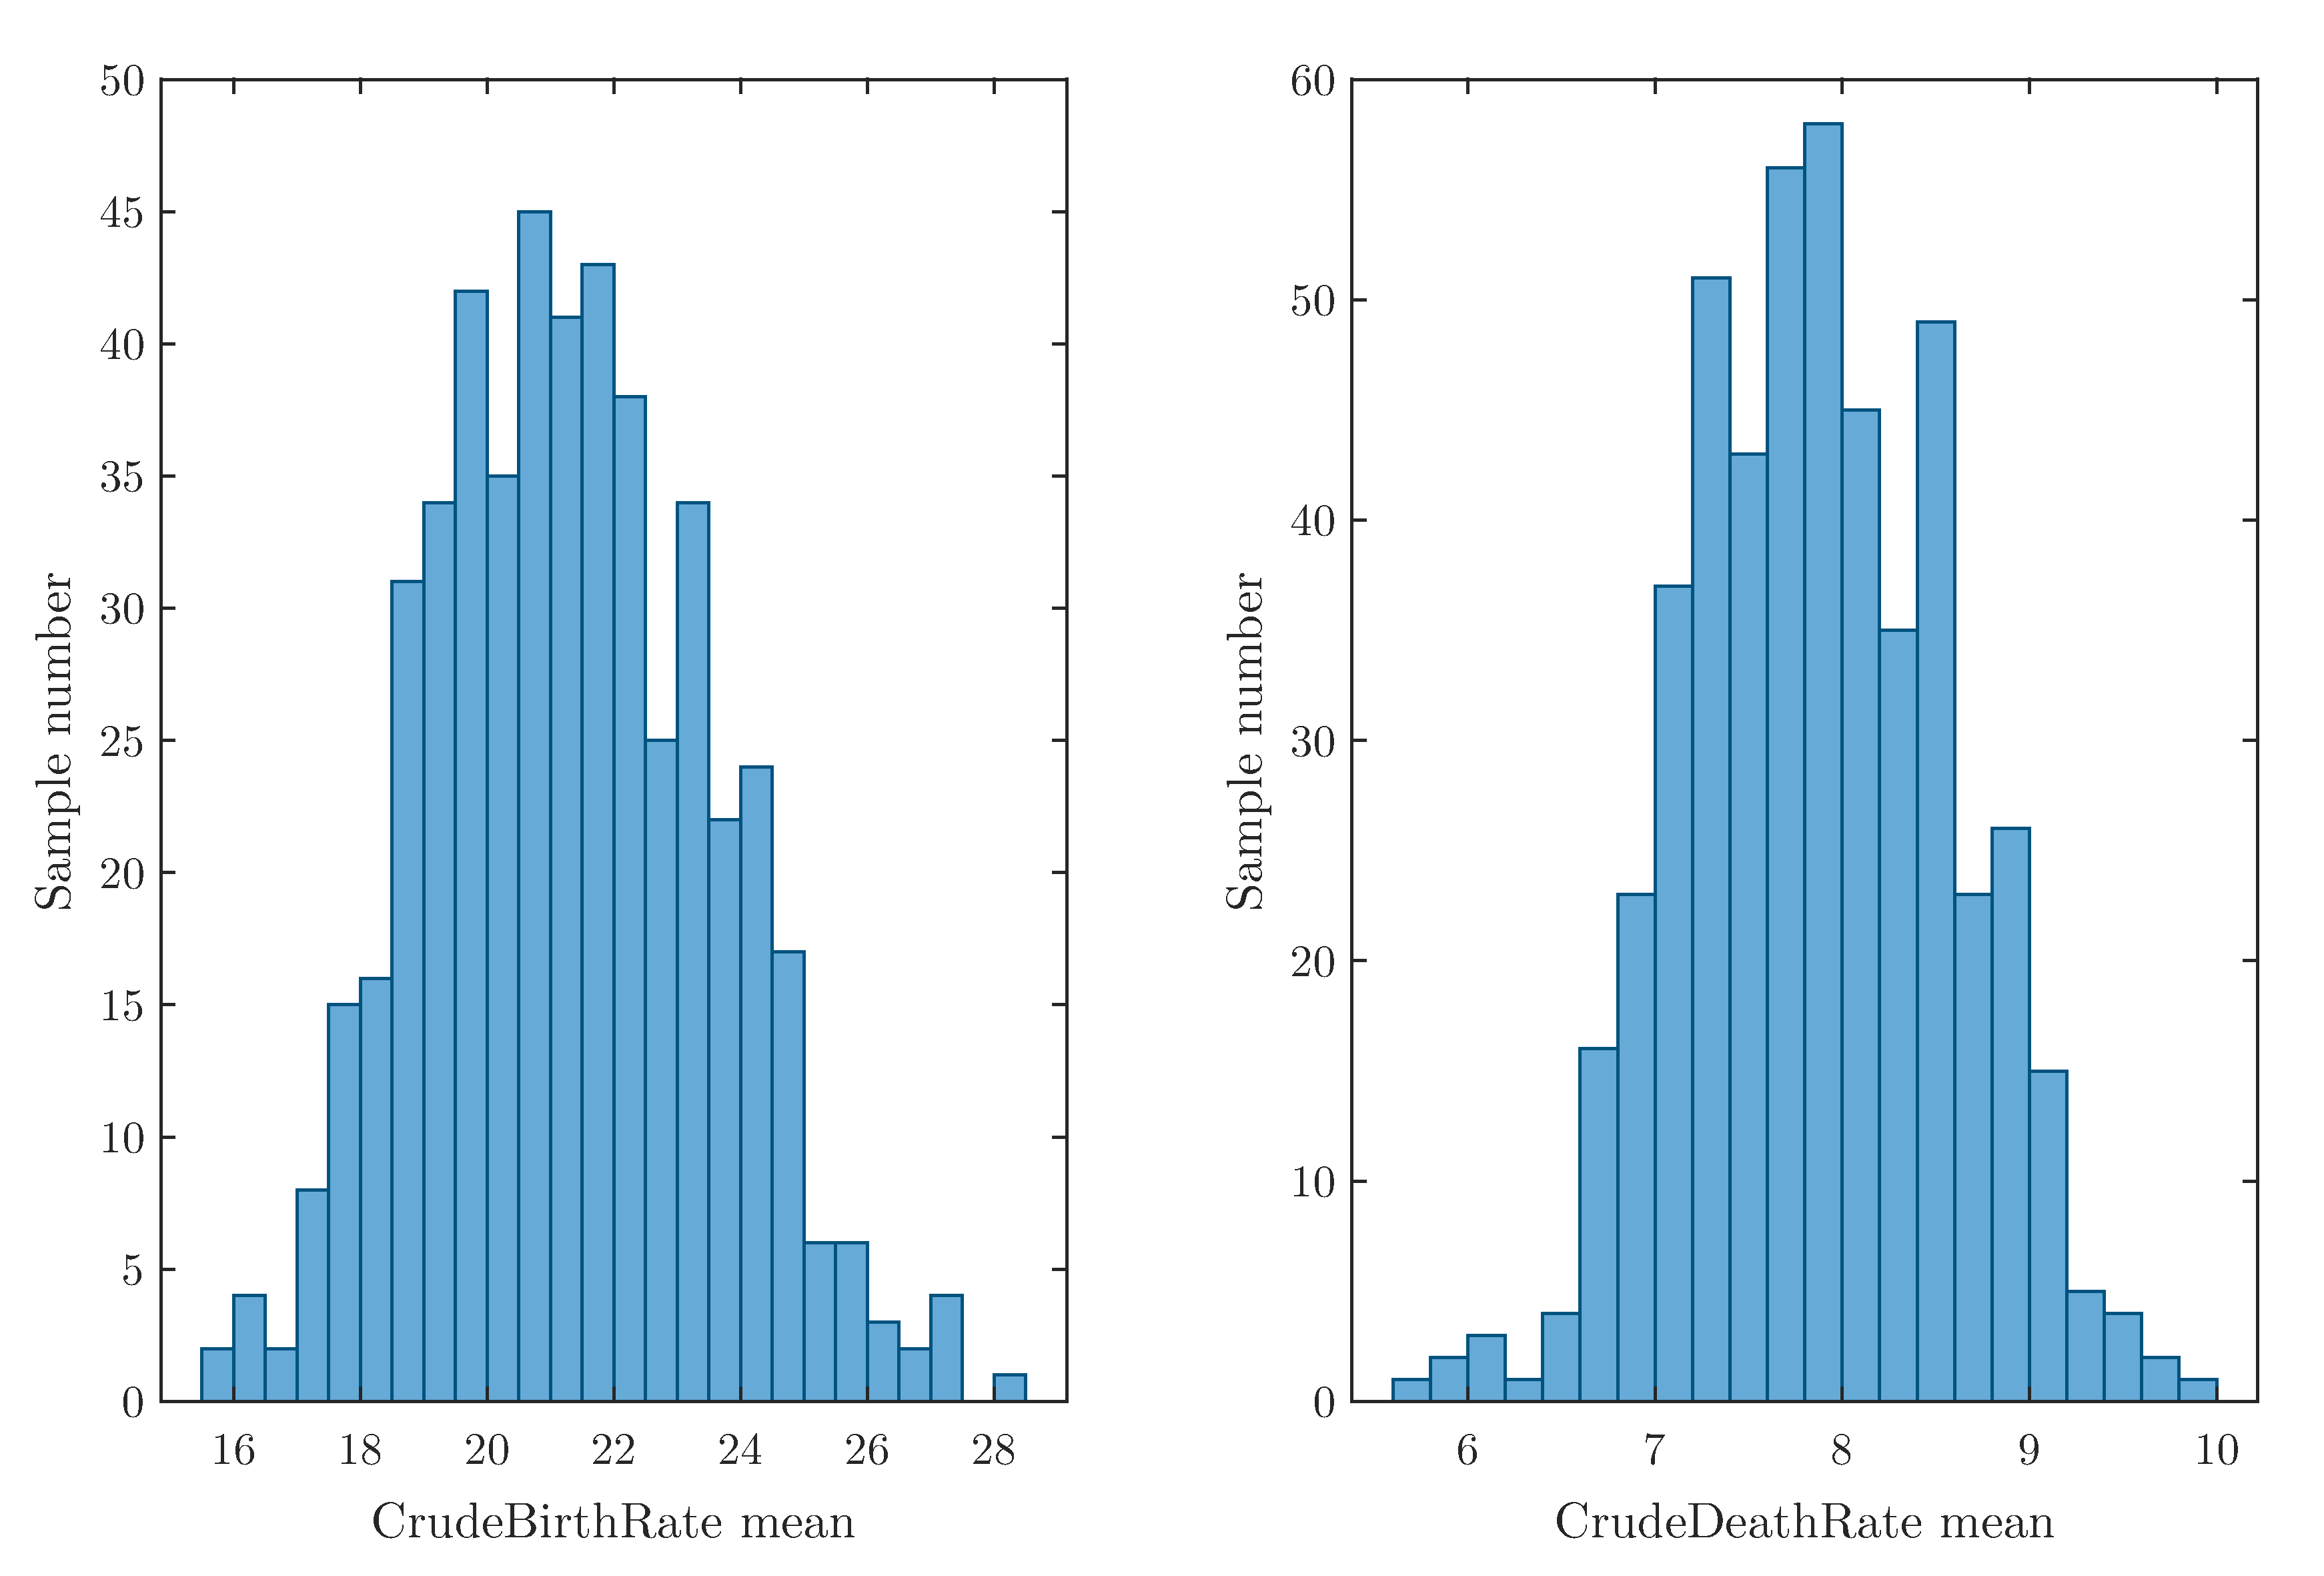
\includegraphics[scale=0.24]{resources/pdf/q2bi.pdf}
		\caption{Histogrammes de $m_{\chi}$ pour $500$ échantillons.}
		\label{figure:Q2bi}
	\end{figure}
	Les moyennes de $m_{\chi}$, reprises dans la table \ref{table:Q2b} avec les autres estimateurs, sont très, voir extrêmement, proches des moyennes de la population. En effet, les erreurs relatives qu'elles comportent sont toutes inférieures au pourcent.
	\subsubsection{Histogrammes de $median_{\chi}$} \label{sec:Q2bii}
	À nouveau, les distributions, représentées par les histogrammes de la figure \ref{figure:Q2bii}, décrivent de manière limpide des lois normales. On notera cependant que celle du taux de natalité présente un pic. \par
	\begin{figure}[h!]
		\centering
		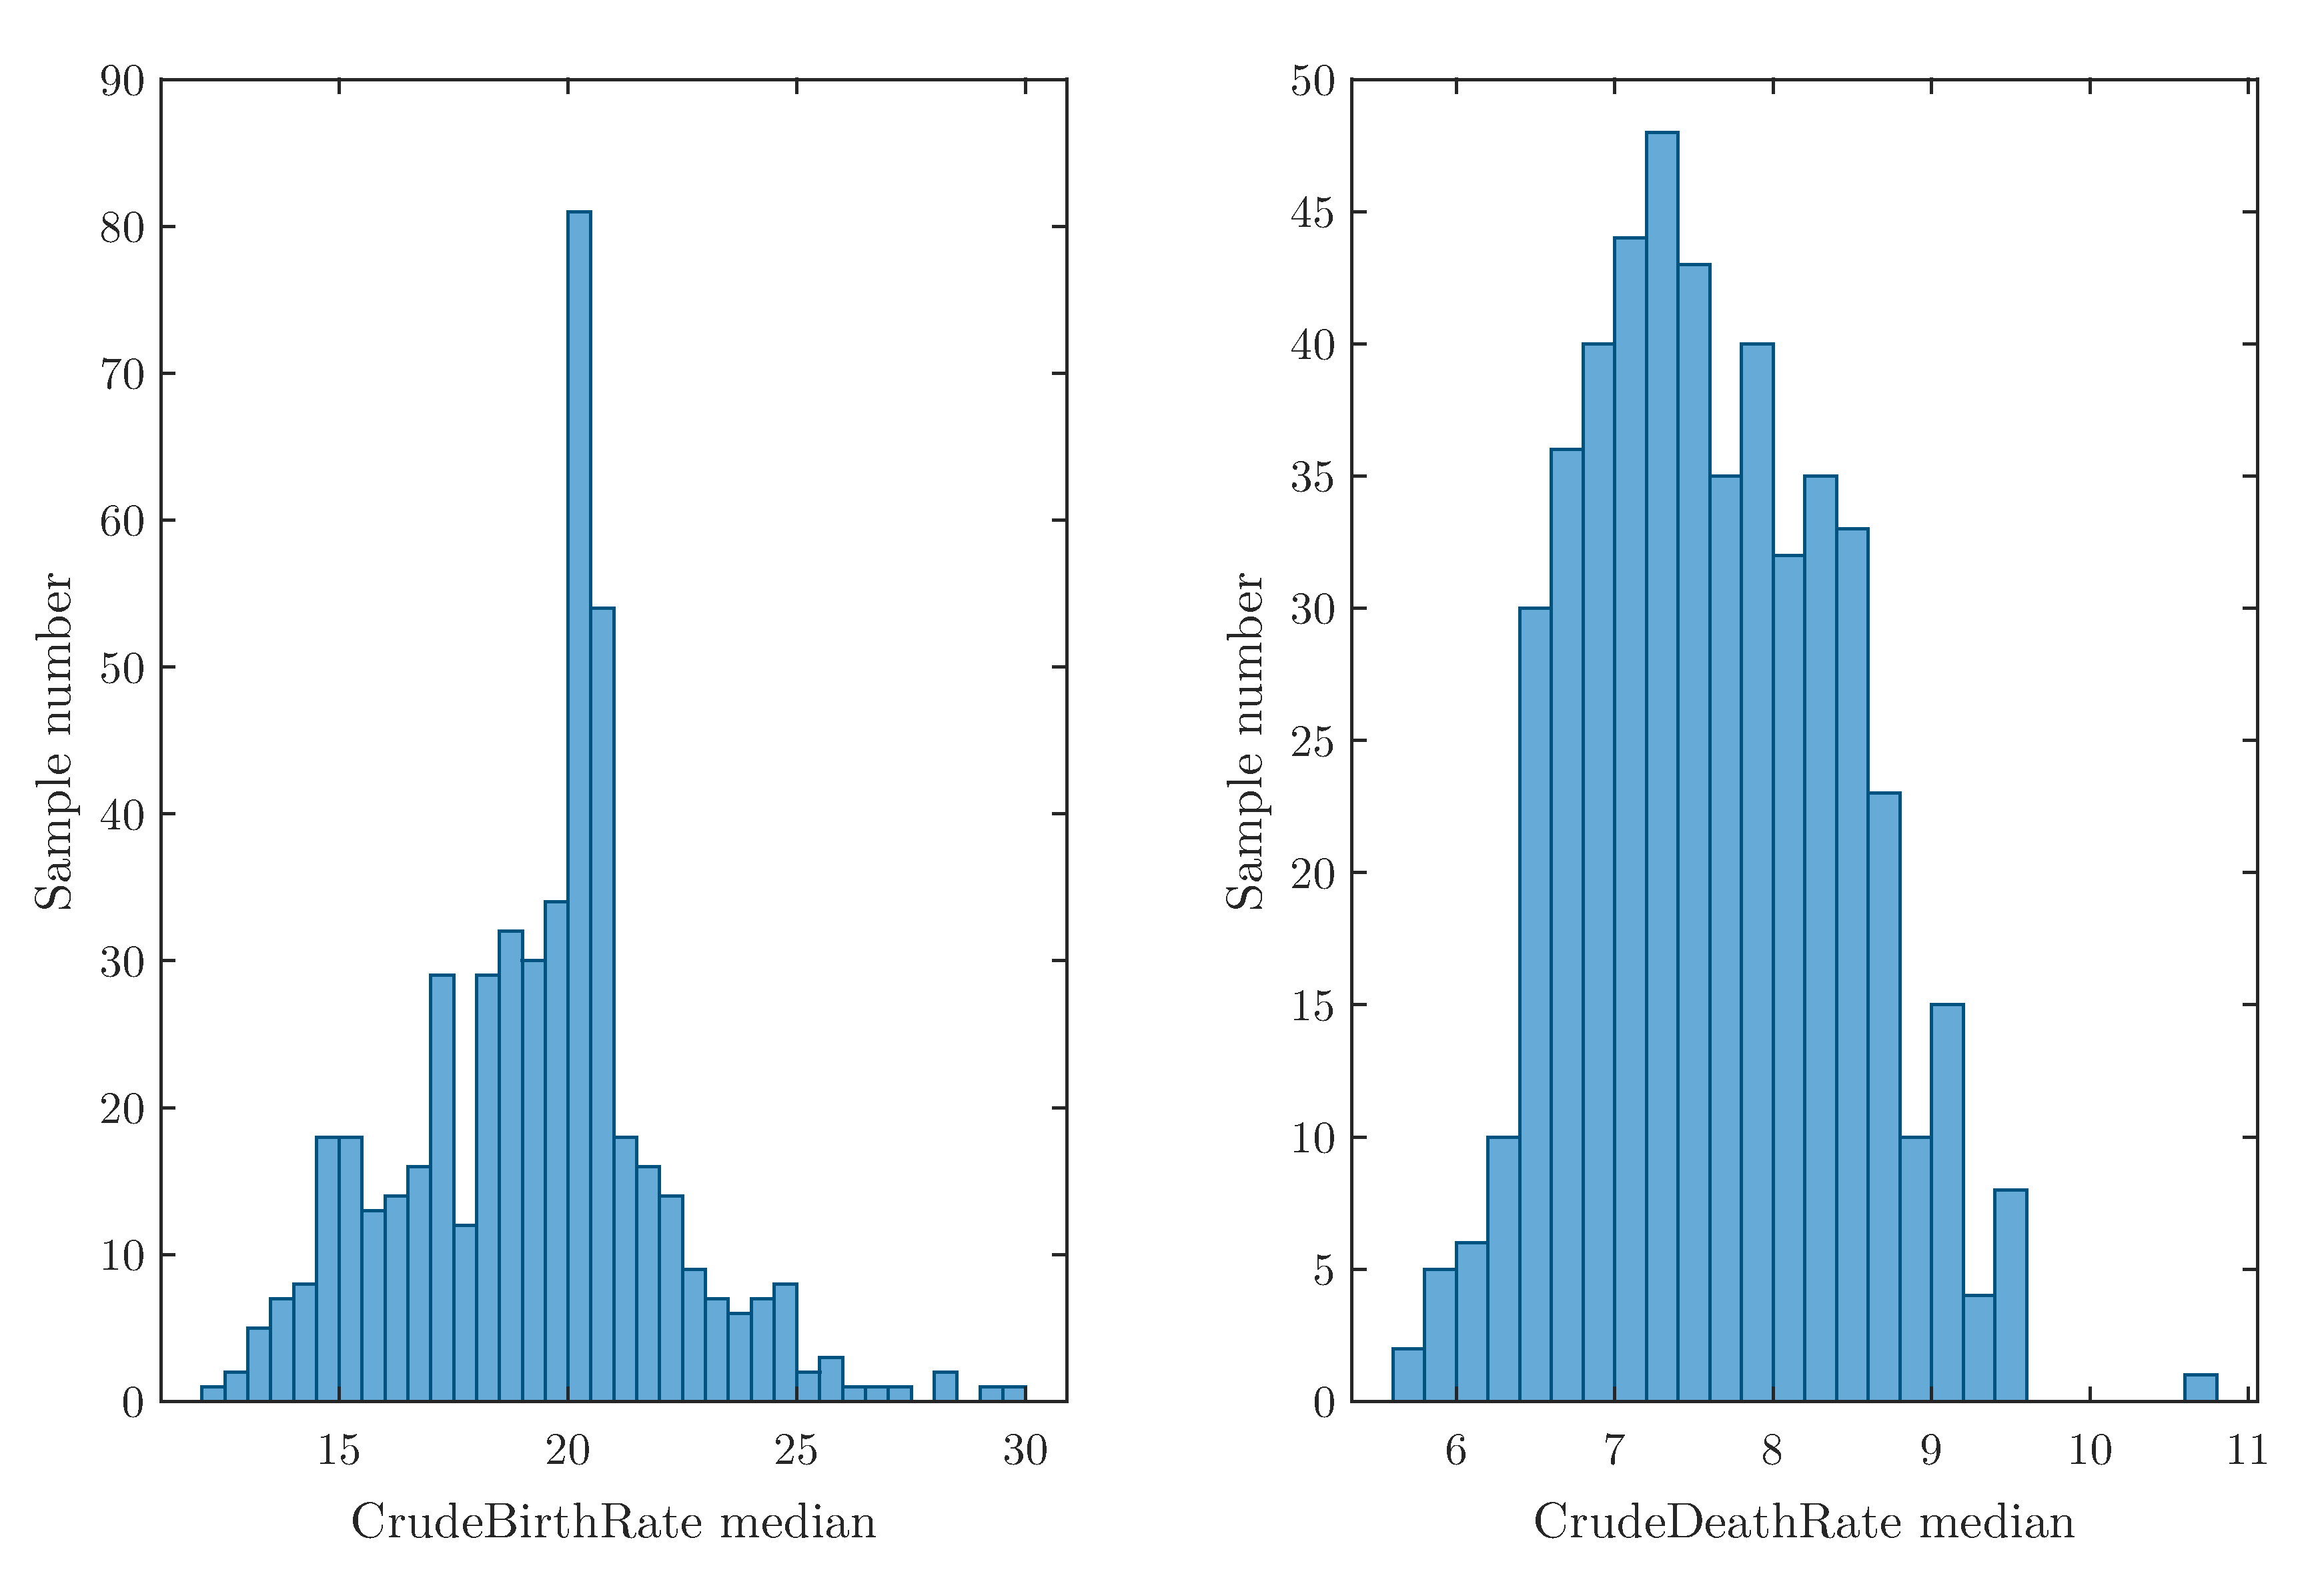
\includegraphics[scale=0.24]{resources/pdf/q2bii.pdf}
		\caption{Histogrammes de $median_{\chi}$ pour $500$ échantillons.}
		\label{figure:Q2bii}
	\end{figure} 
	Cette fois-ci, les moyennes de $median_{\chi}$ sont éloignées des taux médians de la population par des erreurs relatives allant jusqu'à dépasser $3 \%$; un moins bon résultat que $m_{\chi}$. A fortiori, ses moyennes sont plus éloignées encore du taux moyen, qu'elles sous-estiment largement. Néanmoins, ce résultat est parfaitement compréhensible, puisque la médiane de la population sous-estime elle même le taux moyen. La médiane constitue donc un moins bon estimateur du taux moyen que la moyenne. \par
	Théoriquement, il est souvent dit de la médiane qu'elle est un meilleur estimateur que la moyenne. En effet, contrairement à la moyenne, la médiane est généralement peu touchée, et donc peu biaisée, par la présence de valeurs aberrantes. Cependant, dans notre cas, notre population ne contient pas de données aberrantes (cf. section \ref{sec:Q1d}) et, dès lors, la médiane perd son avantage sur la moyenne.
	\subsubsection{Histogrammes de $s_{\chi}$} \label{sec:Q2biii}
	À première vue, on semble reconnaître dans la figure \ref{figure:Q2biii} des lois normales. Cependant, nous savons que la distribution de la variance, \cad le carré de $s_{\chi}$ suit, à un coefficient multiplicatif près, une loi Chi-carré à $n - 1$ degrés de liberté ($\chi^2_{n-1}$). Dès lors, $s_{\chi}$ ne peut pas suivre une loi normale. \par
	\begin{figure}[h!]
		\centering
		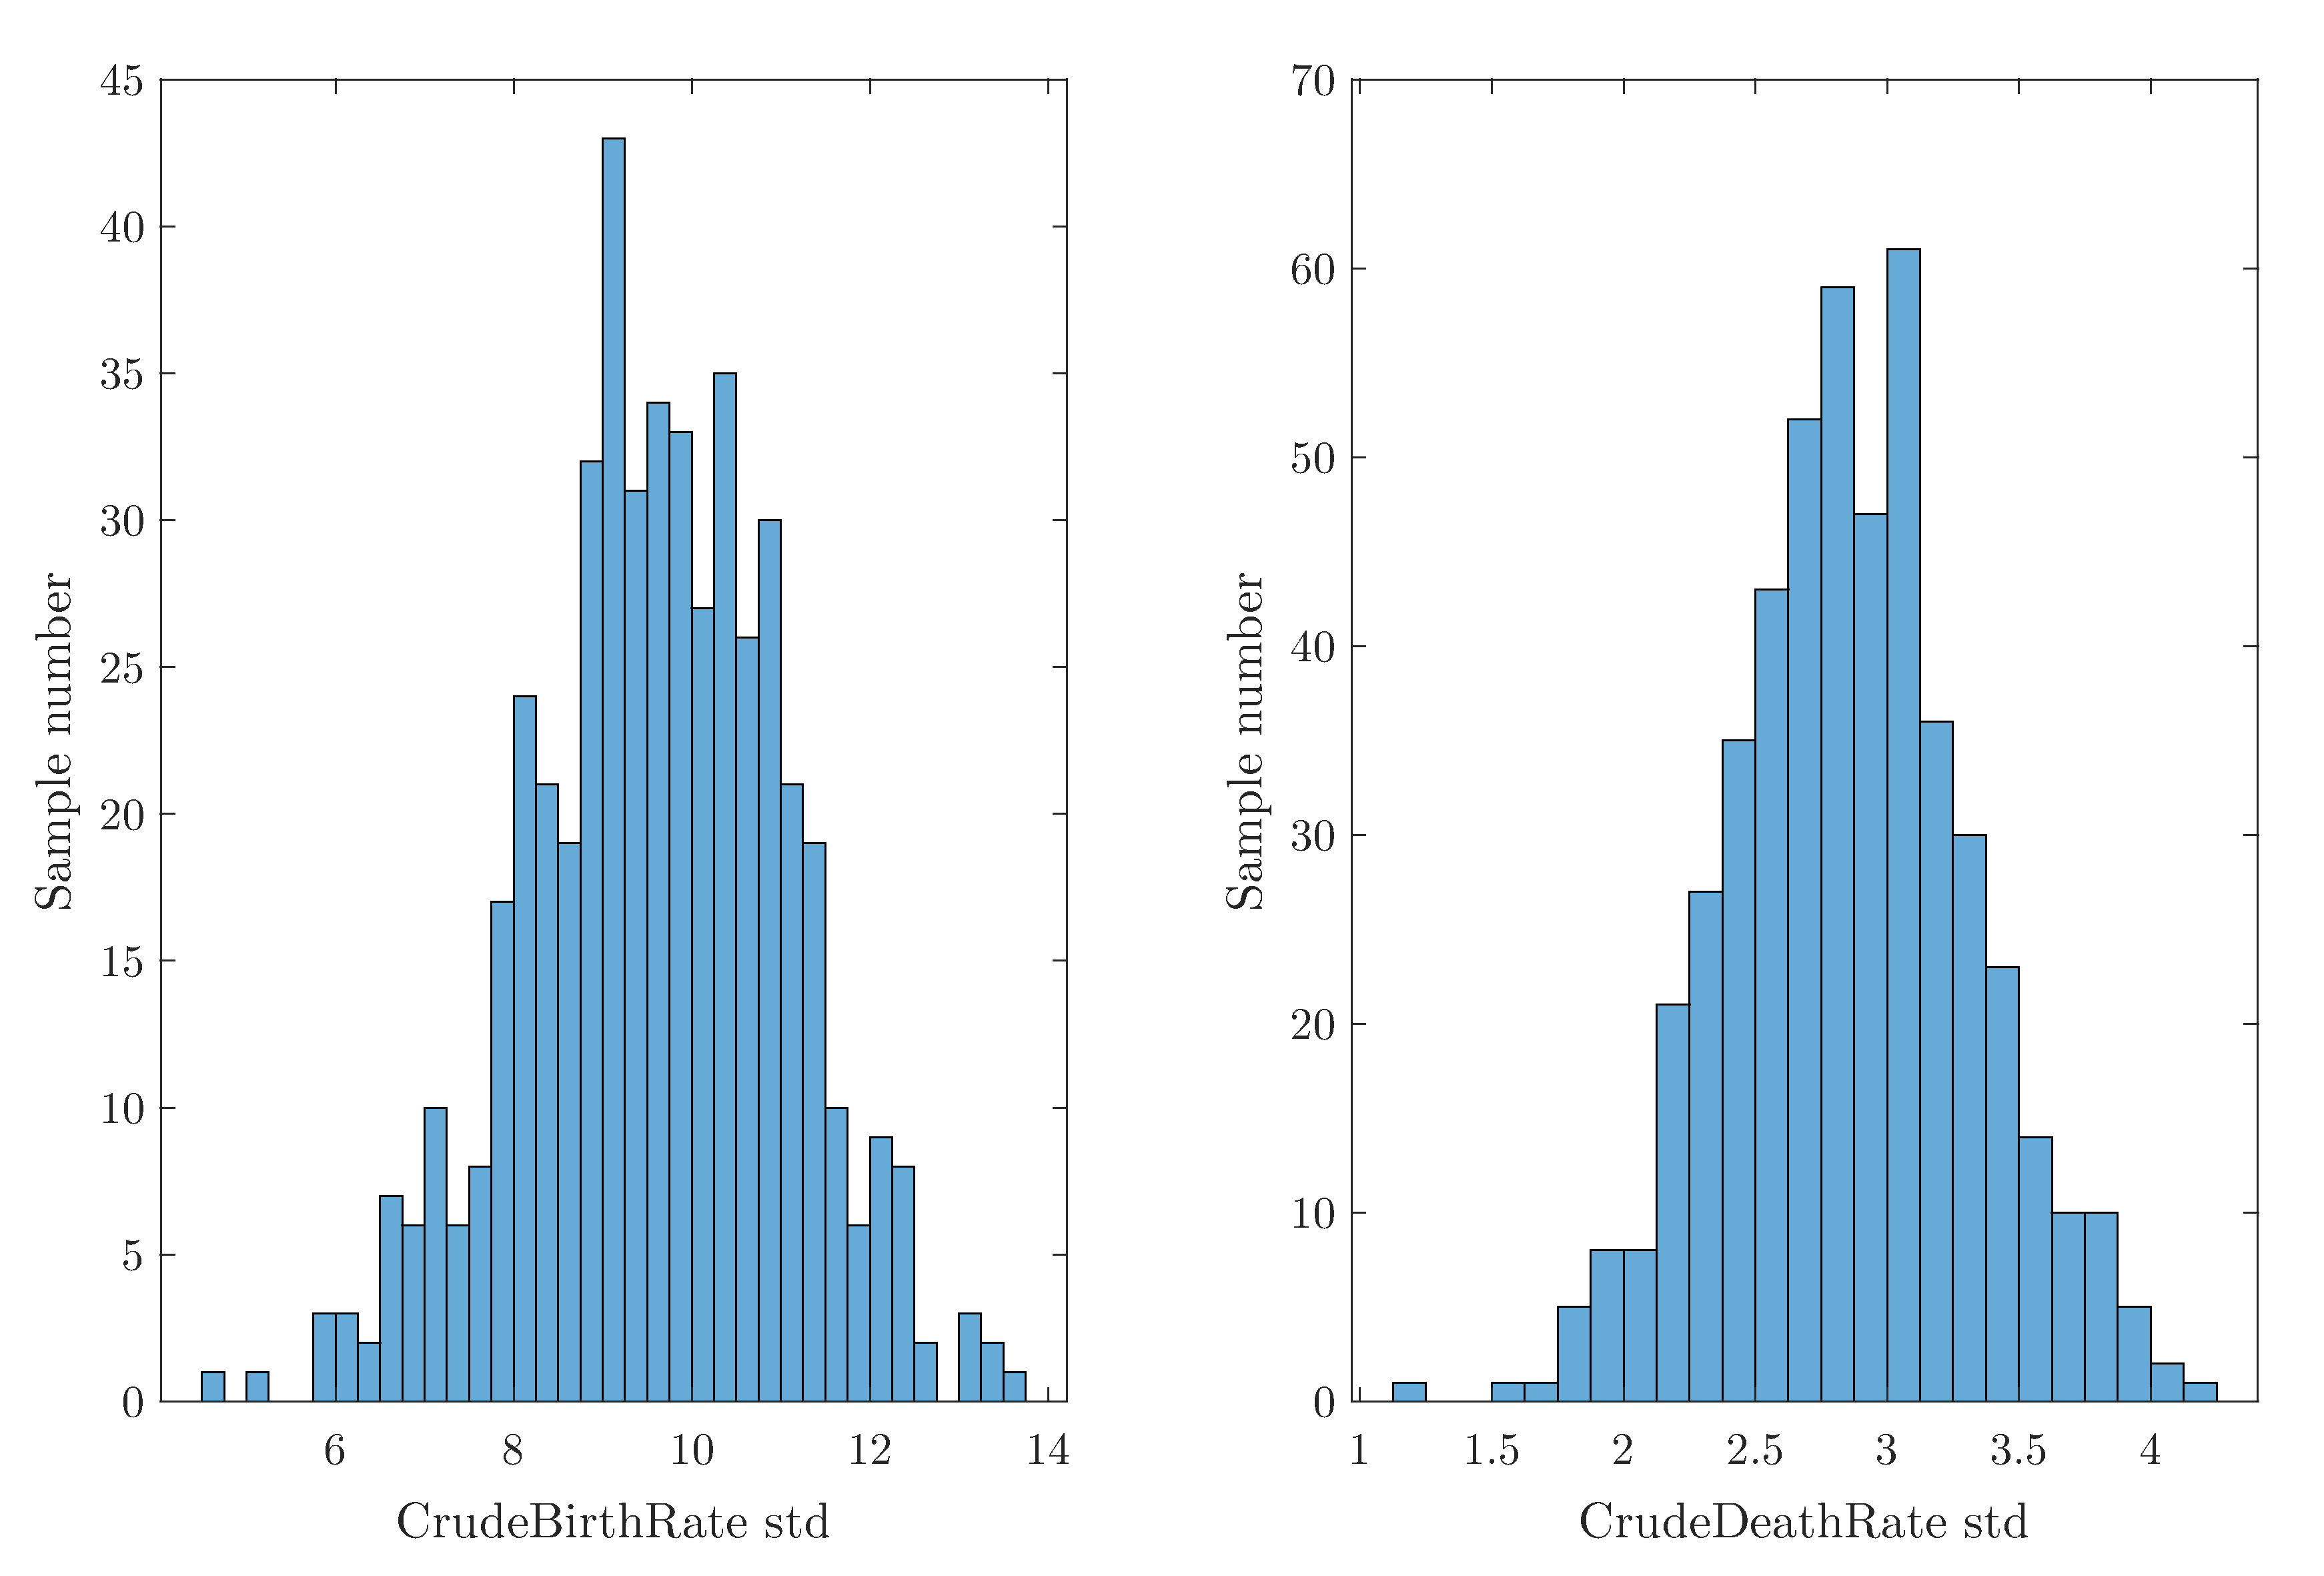
\includegraphics[scale=0.24]{resources/pdf/q2biii.pdf}
		\caption{Histogrammes de $s_{\chi}$ pour $500$ échantillons.}
		\label{figure:Q2biii}
	\end{figure}
	Concernant la moyenne de l'estimateur $s_{\chi}$, on remarque qu'elle sous-estime systématiquement et de manière significative l'écart-type de la population. Cette sous-estimation a déjà été discutée dans le cadre du cours et est le résultat de l'utilisation de la moyenne de l'échantillon à la place de celui de la population dans le calcul de l'écart-type. Pour résoudre ce problème, il suffit d'introduire la correction de Bessel, \cad l'écart-type corrigé\footnote{Son calcul numérique se fait aussi par le biais de la fonction \texttt{std}.}, noté $s_{n-1}$. \par
	Présentes dans la table \ref{table:Q2b}, les moyennes de ce nouvel estimateur sont effectivement beaucoup plus proches de l'écart-type de la population tout en lui restant inférieures. On peut, en effet, prouver à l'aide de l'inégalité de Jensen que $s_{n-1}$ sous-estime l'écart-type de la population.
	\subsubsection{Histogrammes de la distance de Kolmogorov-Smirnov} \label{sec:Q2biv}
	Le calcul des distances de K.-S. est complété par le script \texttt{Q2biv} d'une manière similaire à celle du script \texttt{Q2aiii}. \par
	Bien qu'ils soient à nouveau assimilables à des lois normales, les histogrammes présentés dans la figure \ref{figure:Q2biv} semblent cette fois-ci asymétriques par rapport aux valeurs les plus représentées. \par
	\begin{figure}[h!]
		\centering
		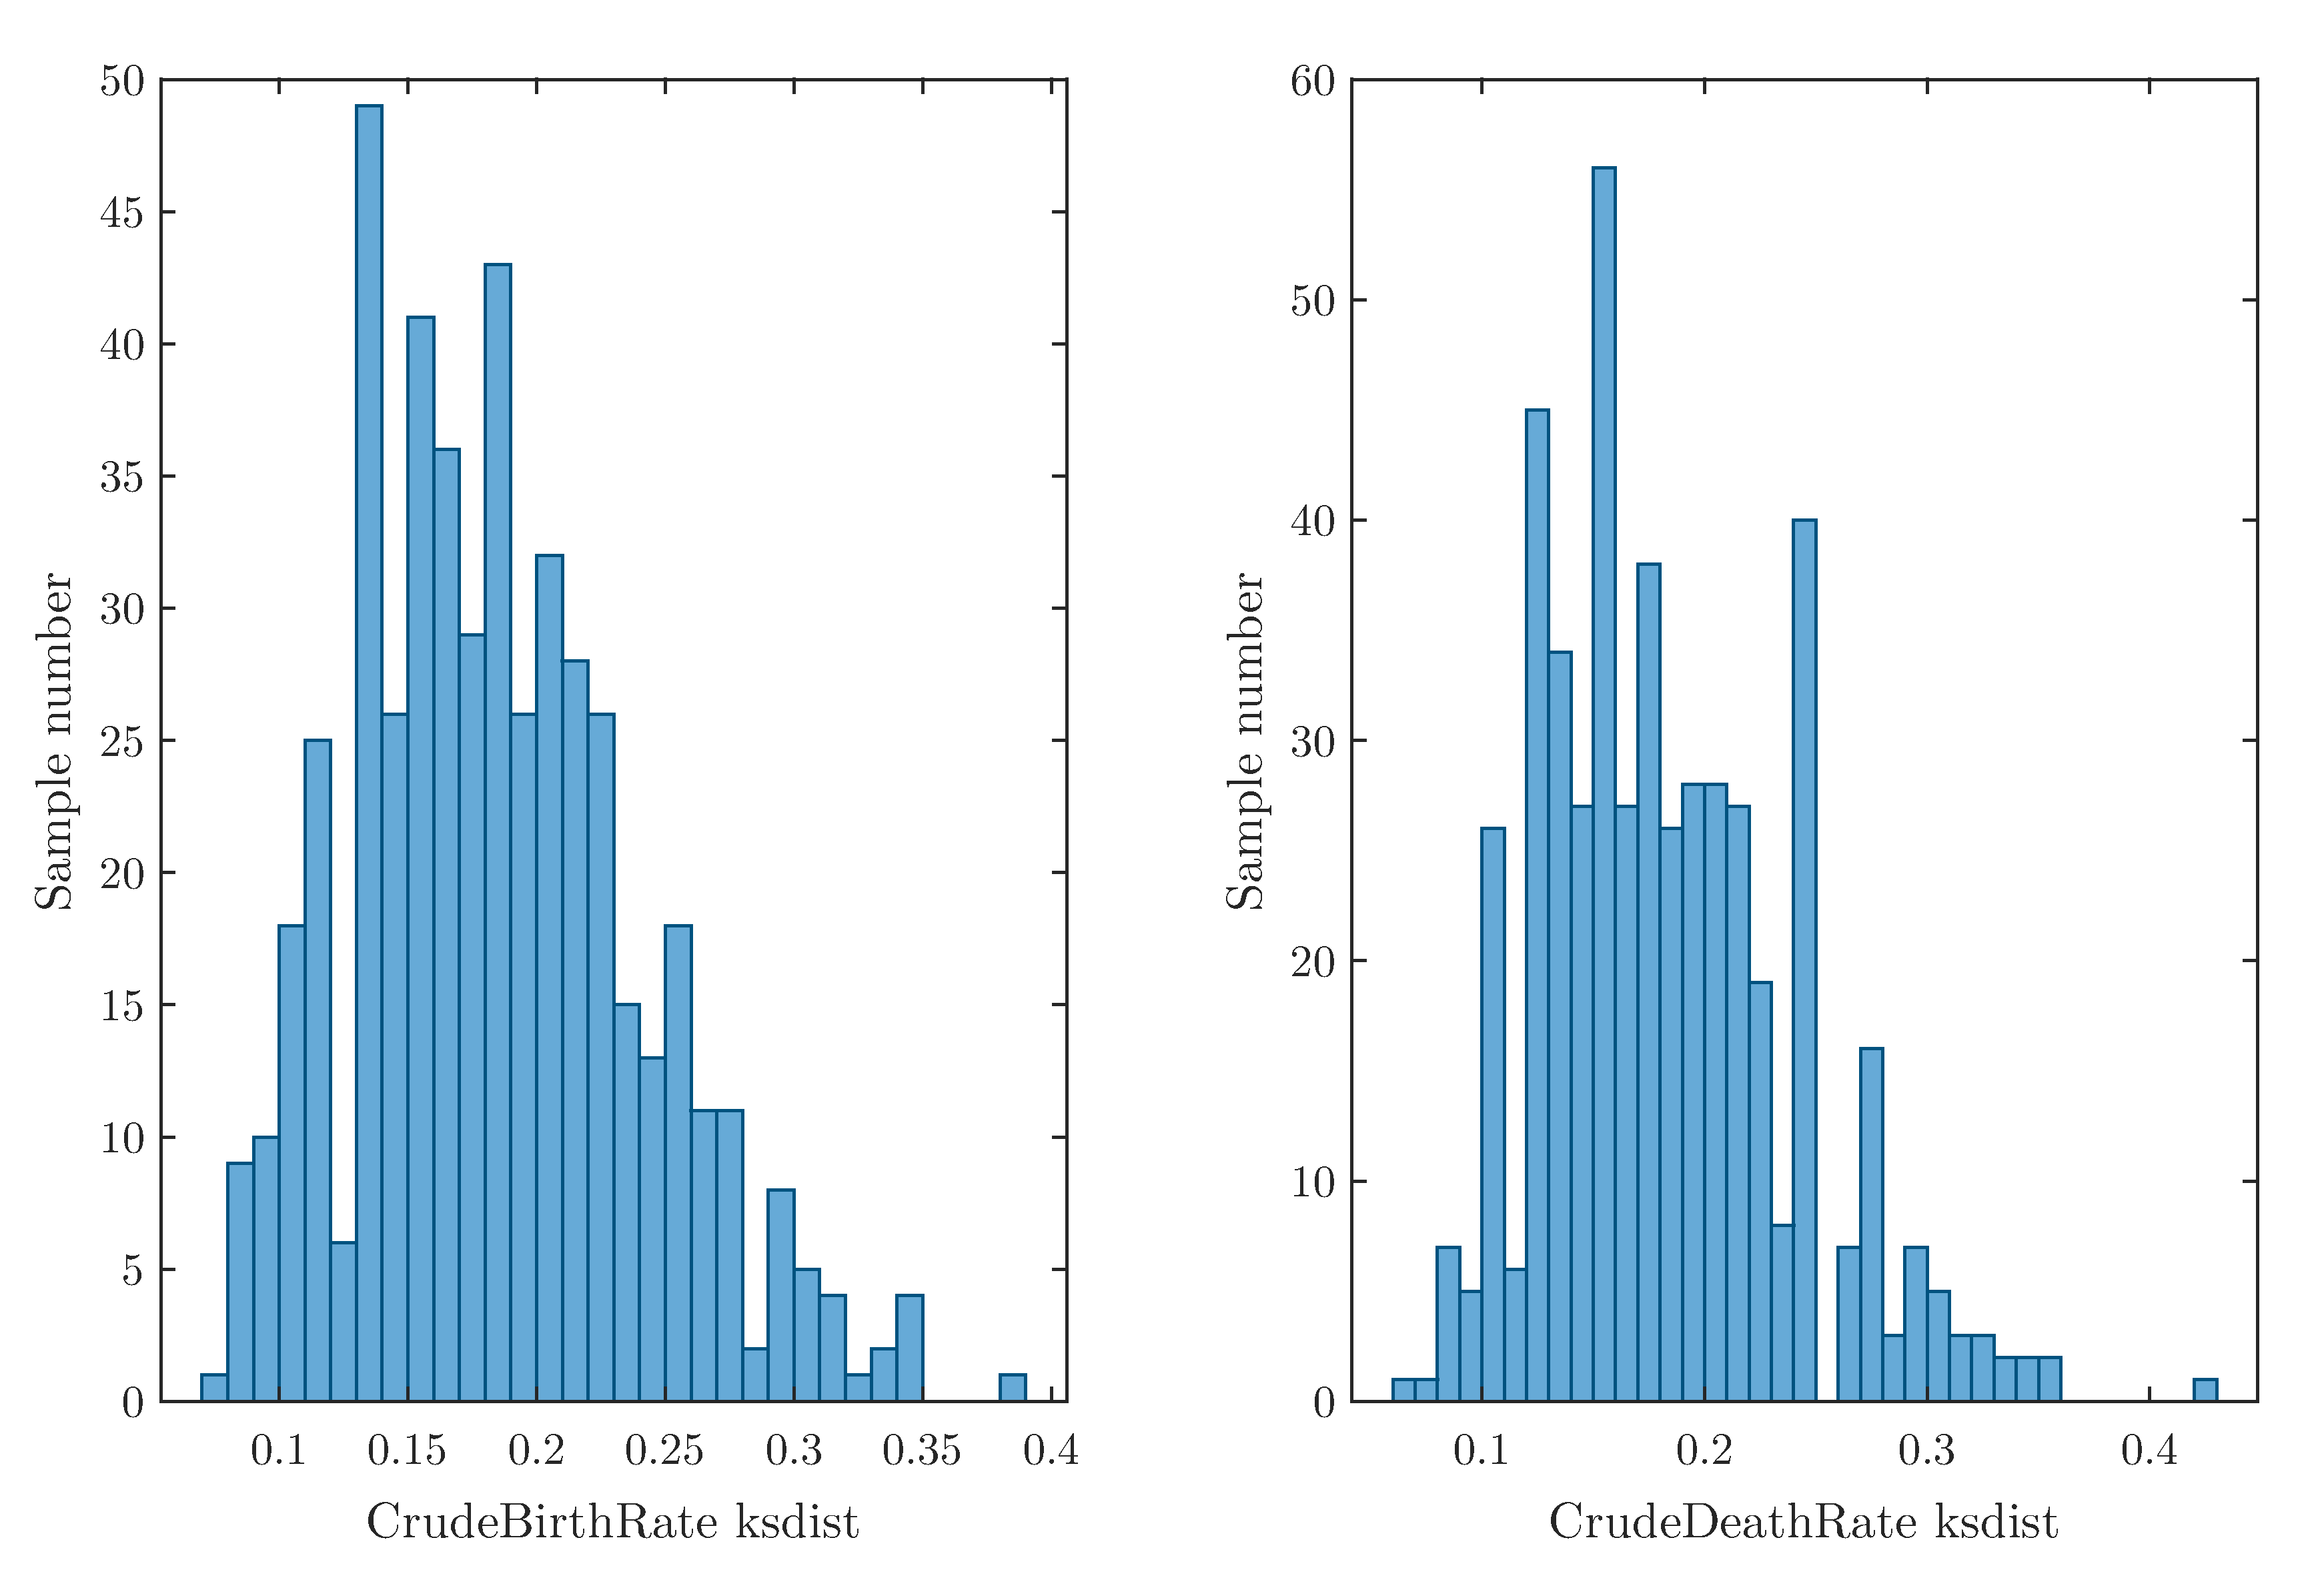
\includegraphics[scale=0.24]{resources/pdf/q2biv.pdf}
		\caption{Histogrammes des distances de Kolmogorov Smirnov entre les polygones des fréquences cumulées des taux pour la population et les échantillons.}
		\label{figure:Q2biv}
	\end{figure}
	\section{Estimation} \label{sec:Q3}
	À partir de maintenant, n'est plus considéré que le taux de natalité. \par
	On souhaite, dans les sections \ref{sec:Q3a}, \ref{sec:Q3b} et \ref{sec:Q3c}, étudier l'impact de la taille des échantillons sur la qualité des estimations de $\mu$, le taux moyen, fournies par la moyenne et la médiane. Ainsi, de façon similaire à la section \ref{sec:Q2b}, le biais (par rapport à $\mu$) et la variance des estimateurs $m_{\chi}$ et $median_{\chi}$ sont déterminés par les scripts \texttt{Q3a2b} et \texttt{Q3c} pour des sets de $100$ échantillons de respectivement $20$ et $50$ pays. \par
	\begin{table}[h]
		\centering
		\begin{tabular}{|c|c|c|c|c|c|}
			\hline
			\multirow{2}{*}{Taille} & \multirow{2}{*}{Set} & \multicolumn{2}{c|}{Biais de [\ptsd]} & \multicolumn{2}{c|}{Variance de [$\text{\ptsd}^2$]} \\ \cline{3-6}
			                        &                      &    $m_{\chi}$    &  $median_{\chi}$   &   $m_{\chi}$   &           $median_{\chi}$           \\ \hline\hline
			  \multirow{3}{*}{20}   &         $1$          & $\num{3.24e-2}$  &   $\num{-1.555}$   & $\num{5.366}$  &            $\num{8.402}$            \\ \cline{2-6}
			                        &         $2$          & $\num{-4.68e-2}$ &   $\num{-2.151}$   & $\num{4.336}$  &            $\num{7.768}$            \\ \cline{2-6}
			                        &         $3$          & $\num{7.02e-2}$  &  $\num{-2.0995}$   & $\num{4.944}$  &            $\num{8.966}$            \\ \hline\hline
			  \multirow{3}{*}{50}   &         $4$          & $\num{-2.07e-2}$ &  $\num{-1.9745}$   & $\num{1.5196}$ &           $\num{2.1314}$            \\ \cline{2-6}
			                        &         $5$          & $\num{2.75e-2}$  &  $\num{-1.9395}$   & $\num{2.6351}$ &           $\num{4.0747}$            \\ \cline{2-6}
			                        &         $6$          & $\num{-4.02e-2}$ &   $\num{-2.034}$   & $\num{2.3859}$ &           $\num{3.9806}$            \\ \hline
		\end{tabular}
		\caption{Biais et variances des estimateurs $m_{\chi}$ et $median_{\chi}$ pour des échantillons du taux de natalité de $20$ et $50$ pays.}
		\label{table:Q3}
	\end{table}
	\subsection{Moyenne} \label{sec:Q3a}
	Comme la section \ref{sec:Q2bi} le laissait présager, on remarque à l'aide de la table \ref{table:Q3} que le biais de l'estimateur $m_{\chi}$ est très faible par rapport à la moyenne de la population. Il est intéressant de noter que le biais peut être positif comme négatif, ce qui traduit une distribution non-biaisée autour du taux moyen. \par
	La variance semble quant à elle orbiter près de la valeur $5$. Il est cependant difficile d'interpréter ce nombre car il représente une distance \og{}au carré\fg{}. Pour interpréter, on utilise donc sa racine, l'écart-type, orbitant autour de $\num{2.2}$. Cette valeur traduit l'étalement de l'estimateur $m_{\chi}$ et est relativement faible.
	\subsection{Médiane} \label{sec:Q3b}
	Il a été dit précédemment que l'estimateur médiane sous-estimait le taux moyen. Ce résultat apparaît nettement dans la table \ref{table:Q3}, le biais étant systématiquement négatif. On notera que ce biais reste proche du biais réel offert par la médiane de la population. \par
	On apprend aussi, grâce à la variance, que la médiane possède une distribution plus étalée que la moyenne.
	\subsection{Échantillons de cinquante pays} \label{sec:Q3c}
	En augmentant la taille des échantillons, deux phénomènes notables se produisent. Le premier est que les biais fluctuent moins et le second que les variances ont diminué. Ce dernier est une conséquence évidente de l'augmentation de la taille des échantillons. \par
	Le premier, quant à lui, décrit la stabilisation, avec la taille des échantillons, de la moyenne des estimateurs. Puisque le biais de l'estimateur $m_{\chi}$ tend vers $0$, on peut dire que sa moyenne tend bien vers le taux moyen. De manière analogue, on attend de la moyenne de l'estimateur $median_{\chi}$ qu'elle tende vers le taux médian. Pour confirmer cette hypothèse, il faut vérifier que le biais de $median_{\chi}$ tende bien vers le biais réel de la médiane de la population. Cependant, bien qu'ils ne s'en soient pas éloignés, les biais pour des échantillons de $50$ pays n'en sont pas réellement plus proches que ceux de $20$ pays. Néanmoins, avec une taille d'échantillon beaucoup plus grande (i.e. $\num{1000}$), cette convergence devient très notable. \par
	Ainsi, il est naturel pour l'estimateur $median_{\chi}$ de sous-estimer le taux moyen puisqu'il estime sans-biais le taux médian, lui étant inférieur.
	\subsection{Intervalles de confiance} \label{sec:Q3d}
	Pour construire les intervalles de confiance associés aux échantillons, il a été fait le choix arbitraire que l'écart-type de la population était inconnu. Dès lors, dans l'hypothèse d'une distribution normale de la variable parente, les bornes des intervalles dépendent des estimateurs $m_{\chi}$ et $s_{n-1}$ :
	\begin{align*}
	    m_{\chi} - x_{1 - \frac{\alpha}{2}} \frac{s_{n-1}}{\sqrt{n}} \leq \mu \leq m_{\chi} + x_{1 - \frac{\alpha}{2}} \frac{s_{n-1}}{\sqrt{n}}
	\end{align*}
	Où $\mu$ est le taux moyen et $x_{1 - \frac{\alpha}{2}}$ est la valeur associée à la proportion $1 - \frac{\alpha}{2}$ par la loi de construction utilisée. En l'occurrence, il est demandé d'utiliser deux lois :
	\begin{enumerate}[noitemsep, label=\roman*.]
	    \item Une loi de student\footnote{Le degré de liberté qu'il faut utiliser est $n-1$, \cad la taille des échantillons réduit d'une unité.} : $x_{1 - \frac{\alpha}{2}} = t_{1 - \frac{\alpha}{2}} =  \num{2.093}$.
	    \item Une loi de Gauss : $x_{1 - \frac{\alpha}{2}} = u_{1 - \frac{\alpha}{2}} = \num{1.96}$.
	\end{enumerate}
	Dans le script \texttt{Q3d}, $x_{1 - \frac{\alpha}{2}}$ est déterminée à l'aide de la fonction \texttt{icdf} qui prend en paramètres une loi parmi celles stockées dans la matrice \texttt{g}, et la proportion $1 - \frac{\alpha}{2}$. Ensuite, la fonction \texttt{hasIn} vérifie pour chaque intervalle construit s'il contient le taux moyen ou non. \par
	\begin{table}[h!]
		\centering
		\begin{tabular}{|c|c|c|}
			\hline
			\multirow{2}{*}{Set} & \multicolumn{2}{c|}{Loi de} \\ \cline{2-3}
			                     &  student   &     Gauss      \\ \hline\hline
			        $1$          & $\num{93}$ &   $\num{92}$   \\ \hline
			        $2$          & $\num{96}$ &   $\num{96}$   \\ \hline
			        $3$          & $\num{97}$ &   $\num{95}$   \\ \hline
		\end{tabular}
		\caption{Nombre d'intervalles contenant $\mu$ pour trois sets de $100$ échantillons de $20$ pays en fonction de la loi utilisée.}
		\label{table:Q3d}
	\end{table}
	On remarque, en premier lieu, que le nombre d'intervalles contenant $\mu$ est toujours plus grand pour la loi de student que pour celle de Gauss. Cela est dû au fait que, pour les mêmes $m_{\chi}$ et $s_{n-1}$, l'intervalle construit avec la loi de student est plus grand que celui construit avec celle de Gauss, car $u_{1 - \frac{\alpha}{2}} \leq t_{1 - \frac{\alpha}{2}}$. \par
	En deuxième lieu, on observe que la proportion d'intervalles rejetés est proche de $\alpha$, ce qui est logique. Cependant, les valeurs obtenues sont parfois supérieures à ce qui est attendu ($\num{95} \,\%$). Cela est dû au hasard de l'échantillonnage. En effet, en augmentant le nombre d'échantillons à $\num{10000}$ (cf. table \ref{table:Q3dbis}), on note que le nombre d'intervalles contenant $\mu$ y est systématiquement inférieur. \par
		\begin{table}[h!]
		\centering
		\begin{tabular}{|c|c|c|}
			\hline
			\multirow{2}{*}{Set} & \multicolumn{2}{c|}{Loi de} \\ \cline{2-3}
			                     &   student    &    Gauss     \\ \hline\hline
			        $1$          & $\num{9413}$ & $\num{9266}$ \\ \hline
			        $2$          & $\num{9420}$ & $\num{9259}$ \\ \hline
			        $3$          & $\num{9419}$ & $\num{9282}$ \\ \hline
		\end{tabular}
		\caption{Nombre d'intervalles contenant $\mu$ pour trois sets de $\num{10000}$ échantillons de $20$ pays en fonction de la loi utilisée.}
		\label{table:Q3dbis}
	\end{table}
	Ce résultat est plus probant et traduit le fait que la distribution de la loi parente, en tout cas dans notre base de donnée, ne suit pas exactement une loi normale, bien qu'elle y raisonnablement assimilable.
	\section{Tests d'hypothèse} \label{sec:Q4}
	Tirer $100$ fois un échantillon de 40 pays par organisme, \cad l'état belge et les quatre instituts, comme il est demandé dans l'énoncé, revient à tirer $\num{500}$ échantillons et les répartir ensuite aléatoirement entre eux. C'est ce qui est implémenté dans le script \texttt{Q4}. \par
	Pour déterminer $x$ et $p$, les proportions de pays ayant un taux de natalité plus faible que la Belgique respectivement dans la population et dans les échantillons, on utilise la fonction \texttt{cf}\footnote{Il est important de remarquer que, sans un paramètre additionnel, \texttt{cf} détermine la proportion des valeurs \og{}plus faible ou égale\fg{}.}. Ce faisant, pour la population, on trouve $x = \num{0.2}$. \par
	Pour vérifier l'hypothèse $H_{0}$, il faut satisfaire à un test d'hypothèse unilatéral à droite pour une proportion. Cela signifie que les proportions $p$ doivent satisfaire l'inégalité
	\begin{align*}
	    p & \leq x + u_{1 - \frac{\alpha}{2}} \sqrt{\frac{x (1 - x)}{n}} \\
	      & \leq \num{0.3240}
	\end{align*}
	Cependant, ce test n'est valide que si on peut assimiler la distribution de la variable $p$ à une loi normale de moyenne $x$ et d'écart-type $\sqrt{x (1 - x)}$, ce qui n'est valable que lorsque $\min{\left(n x; \, n(1 - x)\right)} \geq 5$. Ce dernier critère étant validé, le test l'est aussi. \par
	Ainsi, il suffit de comparer chaque $p$ avec la borne calculée pour déterminer le nombre d'échantillons qui vérifie l'hypothèse nulle. Les résultats de cette comparaison sont fournis dans la table \ref{table:Q4}. \par
	\begin{table}[h!]
		\centering
		\begin{tabular}{|c|c|c|c|c|c|c|}
			\hline
			\multirow{2}{*}{Set} & \multirow{2}{*}{Belgique} & \multicolumn{4}{c|}{Institut} & \multirow{2}{*}{OMS} \\ \cline{3-6}
			                     &                           & $1$ & $2$ & $3$ &     $4$     &                      \\ \hline\hline
			        $1$          &            $4$            & $6$ & $8$ & $2$ &     $0$     &         $15$         \\ \hline
			        $2$          &            $6$            & $5$ & $7$ & $5$ &     $3$     &         $20$         \\ \hline
			        $3$          &            $5$            & $6$ & $6$ & $2$ &     $2$     &         $18$         \\ \hline
		\end{tabular}
		\caption{Nombre de rejets de $H_{0}$ pour trois sets de $5$ fois $100$ échantillons de $40$ pays.}
		\label{table:Q4}
	\end{table}
	\subsection{Comparaison à $\alpha$}
	Le nombre de fois où l'état belge a rejeté l'hypothèse nulle orbite autour de $5$. Puisque $100$ tests ont été effectués, on obtient bien une valeur proche de $\alpha$, \cad $5 \%$. Cependant, on remarque pour les autres instituts que cette valeur fluctue. Pour s'assurer de la proportion proche de $\alpha$ d'hypothèse rejetée, on effectue les tests pour des sets de $5$ fois $\num{10000}$. \par
    \begin{table}[h!]
		\centering
		\begin{tabular}{|c|c|c|c|c|c|c|}
			\hline
			\multirow{2}{*}{Set} & \multirow{2}{*}{Belgique} & \multicolumn{4}{c|}{Institut} & \multirow{2}{*}{OMS} \\ \cline{3-6}
			                     &                           &  $1$  &  $2$  &  $3$  &  $4$  &  \\ \hline\hline
			        $1$          &           $442$           & $438$ & $429$ & $478$ & $429$ &        $1676$        \\ \hline
			        $2$          &           $433$           & $390$ & $467$ & $414$ & $439$ &        $1601$        \\ \hline
			        $3$          &           $439$           & $422$ & $440$ & $426$ & $424$ &        $1611$        \\ \hline
		\end{tabular}
		\caption{Nombre de rejets de $H_{0}$ pour trois sets de $5$ fois $\num{10000}$ échantillons de $40$ pays.}
		\label{table:Q4bis}
	\end{table}
	Les résultats de cette seconde expérience, présentés dans la table \ref{table:Q4bis}, confirment l'impression initiale. On note néanmoins que la proportion est toujours inférieure à $\alpha$; différence probablement due à l'hypothèse d'une loi normale.
	\subsection{Considération de l'OMS}
	Sur les trois sets de $100$ échantillons, l'OMS considére, en moyenne, $\num{17.7}$ fois que la Belgique a un taux de natalité faible. Ce nombre de rejets est beaucoup plus élevé que celui fourni par l'état belge. Néanmoins, cela est compréhensible. Il suffit d'un seul rejetant l'hypothèse pour que l'OMS le fasse à son tour. Ainsi, en supposant que, comme la Belgique, chaque institut rejette $H_0$ avec une probabilité $\alpha$, l'OMS le fera avec une probabilité
	\begin{align*}
	    p_4 & = 1 - C^0_4 (1 - \alpha)^{4} = \num{0.1855} \simeq 4 \alpha
	\end{align*}
	En observant les proportions de rejets de l'OMS dans les deux tableaux précédents, on trouve effectivement des valeurs qui en sont proches.
	\subsection{Équilibrage}
	Pour réduire la différence entre la proportion de rejets de l'état belge et celle l'OMS, il faut réduire l'avantage qu'ont, par leur nombre, les instituts. Plusieurs méthodes permettent d'obtenir ce résultat :
	\begin{itemize}
	    \item Puisque le nombre d'instituts, \texttt{ni} dans le code, est leur principal avantage, diminuer ce dernier est une solution. Notamment, on peut déterminer la proportion de rejets de l'OMS pour $3$ et $2$ instituts, respectivement.
	    \begin{align*}
	        p_3 & = 1 - C^0_3 (1 - \alpha)^{3} = \num{0.1426} \simeq 3 \alpha \\
	        p_2 & = 1 - C^0_2 (1 - \alpha)^{2} = \num{0.0975} \simeq 2 \alpha
	    \end{align*}
	    \item Augmenter la tolérance, \texttt{tol} dans le code, de l'OMS est aussi une solution valable. En effet, s'il faut maintenant au moins deux instituts rejetant l'hypothèse pour que l'OMS le fasse, on a comme proportion
	    \begin{align*}
	        p_4' & = 1 - C^0_4 (1 - \alpha)^{4} - C^1_4 \alpha (1 - \alpha)^{3} = \num{0.0140} < \alpha
	    \end{align*}
	    Néanmoins cette proportion est plus faible encore que celle de l'état belge, qui en devient avantagé.
	    \item Diminuer le seuil de signification des instituts ou augmenter celui de Belgique sont aussi des solutions valables.
	\end{itemize}
	\newpage
	\appendix
	\renewcommand{\thesubsection}{\thesection.\arabic{subsection}}
	\section{Ligne de conduite}
	\subsection{Cohérence} \label{sec:Cohérence}
	Dans un soucis de cohérence, chaque script répondant à une question est partitionné de la même manière. Premièrement, dans la section \texttt{Parameters} se trouvent les paramètres liés à la question, comme la taille ou le nombre des échantillons. Ensuite, la section \texttt{Calls} appelle d'autres scripts dont l'utilisation est récurrente. Cela permet de rendre les codes plus concis. Vient après la section \texttt{Compute} qui est le corps principal du script. C'est là que sont effectués les calculs. \par
	Finalement, les sections \texttt{Plot} et \texttt{Display} servent à afficher respectivement les graphiques et les résultats numériques.
	\subsection{Modularité} \label{sec:Modularité}
	Pour rendre le code plus modulaire, l'appel de fonctions calculant une statistique sur un ensemble de données se fait via une matrice (\texttt{f} ou \texttt{g}). Dans cette matrice chaque ligne représente une fonction qui doit être appelée et contient, dans l'ordre, un nom arbitraire associé, le nom d'appel de la fonction et ses paramètres optionnels. Il suffit dès lors d'itérer sur les lignes de cette matrice pour calculer chaque statistique.
	\section{Scripts}
	\lstinputlisting[style=Matlab, caption={\texttt{startup.m}}]{resources/matlab/startup.m}
    \lstinputlisting[style=Matlab, caption={\texttt{loadData.m}}]{resources/matlab/loadData.m}
    \lstinputlisting[style=Matlab, caption={\texttt{pickSamples.m}}]{resources/matlab/pickSamples.m}
    \lstinputlisting[style=Matlab, caption={\texttt{Q1a.m}}]{resources/matlab/Q1a.m}
    \lstinputlisting[style=Matlab, caption={\texttt{Q1b.m}}]{resources/matlab/Q1b.m}
    \lstinputlisting[style=Matlab, caption={\texttt{Q1c.m}}]{resources/matlab/Q1c.m}
    \lstinputlisting[style=Matlab, caption={\texttt{Q1d.m}}]{resources/matlab/Q1d.m}
    \lstinputlisting[style=Matlab, caption={\texttt{Q1e.m}}]{resources/matlab/Q1e.m}
    \lstinputlisting[style=Matlab, caption={\texttt{Q1f.m}}]{resources/matlab/Q1f.m}
    \lstinputlisting[style=Matlab, caption={\texttt{Q2ai.m}}]{resources/matlab/Q2ai.m}
    \lstinputlisting[style=Matlab, caption={\texttt{Q2aii.m}}]{resources/matlab/Q2aii.m}
    \lstinputlisting[style=Matlab, caption={\texttt{Q2aiii.m}}]{resources/matlab/Q2aiii.m}
    \lstinputlisting[style=Matlab, caption={\texttt{Q2b.m}}]{resources/matlab/Q2b.m}
    \lstinputlisting[style=Matlab, caption={\texttt{Q2bhist.m}}]{resources/matlab/Q2bhist.m}
    \lstinputlisting[style=Matlab, caption={\texttt{Q2bi.m}}]{resources/matlab/Q2bi.m}
    \lstinputlisting[style=Matlab, caption={\texttt{Q2bii.m}}]{resources/matlab/Q2bii.m}
    \lstinputlisting[style=Matlab, caption={\texttt{Q2biii.m}}]{resources/matlab/Q2biii.m}
    \lstinputlisting[style=Matlab, caption={\texttt{Q3a2b.m}}]{resources/matlab/Q3a2b.m}
    \lstinputlisting[style=Matlab, caption={\texttt{Q3c.m}}]{resources/matlab/Q3c.m}
    \lstinputlisting[style=Matlab, caption={\texttt{Q3d.m}}]{resources/matlab/Q3d.m}
    \lstinputlisting[style=Matlab, caption={\texttt{Q4.m}}]{resources/matlab/Q4.m}
    \newpage
    \section{Fonctions}
    Lors de l'écriture des fonctions, nous avons fait le choix de ne pas les rendre robustes, \cad que nous supposons leurs entrées valides et ne les vérifions pas.
    \lstinputlisting[style=Matlab, caption={\texttt{cf.m}}]{resources/matlab/cf.m}
    \lstinputlisting[style=Matlab, caption={\texttt{gap.m}}]{resources/matlab/gap.m}
    \lstinputlisting[style=Matlab, caption={\texttt{hasIn.m}}]{resources/matlab/hasIn.m}
    \lstinputlisting[style=Matlab, caption={\texttt{isIn.m}}]{resources/matlab/isIn.m}
    \lstinputlisting[style=Matlab, caption={\texttt{ks2stat.m}}]{resources/matlab/ks2stat.m}
\end{document}